%% Manuscript for submission to Springer journal
%% Based on sn-article template — Basic Author-Year Reference Style
%% ============================================================

\documentclass[pdflatex,sn-basic]{sn-jnl}

\usepackage{graphicx}
\usepackage{amsmath,amssymb,amsfonts}
\usepackage{booktabs}
\usepackage[utf8]{inputenc}
\usepackage[T1]{fontenc}

\raggedbottom

\begin{document}

\title[Field-parameterised $K_{\mathrm{plint}}$ correction factor for Plinthosol erodibility]{A field-parameterised multiplicative correction factor \texorpdfstring{$K_{\mathrm{plint}}$}{K-plint} for USLE erodibility of tropical Plinthosols: formulation, sensitivity analysis and computational validation}

\author*[1]{\fnm{Emersson Guedes} \sur{da Silva}}\email{academicoguedes@gmail.com}

\affil*[1]{\orgdiv{Departamento de Zootecnia},
           \orgname{Universidade Federal de Sergipe},
           \orgaddress{\city{S\~{a}o Crist\'{o}v\~{a}o},
                       \state{SE},
                       \postcode{49100-000},
                       \country{Brazil}}}

\abstract{The erodibility of tropical Plinthosols affected by linear erosion is amplified by subsurface hydraulic impedance, aluminium toxicity and geotechnical vulnerability, convergent processes not captured by the surface attributes of the conventional $K$-factor nomograph.  This study evaluates the mathematical identifiability and physical consistency of a multiplicative correction factor that translates these three mechanisms as independent amplifiers of $K$, totalling five free calibratable parameters.  Five computational tests were conducted using field-measured properties of a Haplic Plinthosol (basic infiltration rate determined by double-ring infiltrometer, 1.53--3.13~cm/h; aluminium saturation from routine chemical analysis, 15--99\%; geotechnical parameters from direct-shear testing, critical height 3.35~m; six erosion features mapped in situ) together with virtual profiles of a Ferralsol and an Acrisol parameterised from regional literature.  Synthetic calibration recovered three of the five parameters with bias below 15\%, whereas the two geotechnical parameters exhibited equifinality mitigable by physical constraint.  Sobol sensitivity analysis indicated that the hydraulic term governs 63--78\% of the amplification variance in the Plinthosol, while the toxicity term dominates 70\% in the Ferralsol, confirming coherence between parametric hierarchy and dominant pedological mechanism.  The Plinthosol generated a runoff coefficient of 0.56 under 60~mm/h intensity (effective conductivity 0.50~cm/h) versus zero runoff in the Ferralsol across all tested intensities, validating the basic infiltration rate threshold of 6~cm/h.  The multiplicative structure may be considered sufficiently robust to support field calibration.}

\keywords{soil erodibility, USLE correction factor, Plinthosol, sensitivity analysis, computational validation, Green--Ampt, slope stability}

\maketitle

%% ================================================================
%%  1. INTRODUCTION
%% ================================================================
\section{Introduction}
\label{sec:intro}

Accelerated water erosion constitutes one of the most severe threats to global agricultural sustainability, with soil loss rates on cultivated land exceeding pedogenesis by one to two orders of magnitude across diverse tropical and subtropical regions \citep{montgomery_2007}. Recent estimates indicate that land-use change may amplify global erosion by up to 14\% by 2050 \citep{borrelli_et_al_2017}, while erosion-driven degradation already compromises the productive capacity of soils across more than one billion hectares \citep{lal_2001}. The magnitude of the problem makes predictive tools indispensable for conservation planning at both catchment and plot scales.

The Universal Soil Loss Equation and its revised version \citep{wischmeier_smith_1978,renard_et_al_1997} remain the most widely used empirical framework for estimating sheet and rill erosion \citep{alewell_et_al_2019}. The erodibility factor ($K$) synthesises the intrinsic susceptibility of the soil, yet its estimation via the nomograph of \citet{wischmeier_et_al_1971} depends exclusively on surface-layer attributes such as particle-size distribution, organic matter, structure and permeability \citep{roemkens_et_al_1997}.

This restriction imposes predictive limitations in tropical soils whose oxidic mineralogy generates aggregation patterns distinct from the temperate Mollisols for which the nomograph was developed \citep{alewell_et_al_2019,cassol_et_al_2023}, resulting in $K$ estimates that frequently diverge by up to one order of magnitude under field conditions on conservation plots in Brazil \citep{silva_et_al_2009,lafayette_cantalice_coutinho_2011}. In Plinthosols affected by linear erosion features, the nomograph discrepancy is amplified by the convergence of three processes absent from the original formulation. Plinthic horizons with cemented concretions reduce saturated hydraulic conductivity to restrictive levels ($<$\,2~cm/h), inducing profile saturation and surface runoff under moderate rainfall events \citep{wang_et_al_2020,embrapa_2018,horton_1933,bertoni_lombardi_neto_2017}; subsurface aluminium saturation suppresses root development and reduces vegetation cover \citep{gura_et_al_2022}; and the evolution from rills to gullies shifts the dominant soil-loss mechanism towards lateral block collapse, headcut retreat and piping \citep{poesen_2018,poesen_et_al_2003,kirkby_bracken_2009,vanmaercke_et_al_2021}. Physically based models capture this erosive continuum \citep{nearing_et_al_1989,sidorchuk_2006}, but the density of their parameterisation limits operational application in data-scarce settings \citep{wilkinson_et_al_2024}.

An alternative that preserves operational applicability consists of correcting the nomograph $K$ via multiplicative factors representing the subsurface processes absent from the original formulation \citep{alewell_et_al_2019}. Models with multiple coupled factors, however, accumulate structural uncertainty, making it indispensable to evaluate the sensitivity and identifiability of their parameters before field calibration \citep{saltelli_et_al_2004}. Sobol global variance-based analysis allows quantification of the individual and interactive contribution of each parameter, identifying redundancies and equifinalities that would remain hidden under local approaches \citep{sobol_2001,francois_et_al_2024}.

The Haplic Plinthosol of the Coastal Tablelands of Sergipe (northeastern Brazil) combines the three amplification mechanisms across wide ranges --- basic infiltration rate (VIB) of 1.53--3.13~cm/h, aluminium saturation of 15--99\% and $H/H_c$ ratio of 0.12--0.45 --- which supports the formulation of a multiplicative correction factor with five free parameters distributed across three independent terms ($K_{\mathrm{plint}} = K_{\mathrm{RUSLE}} \times \alpha(\mathrm{VIB}) \times \beta(m_{\mathrm{Al}}) \times \gamma(H/H_c)$). Because direct calibration of multivariate models requires prolonged monitoring and high instrumental density \citep{alewell_et_al_2019}, prior computational verification of parametric identifiability and physical consistency is a necessary condition for justifying the experimental investment.

To the best of our knowledge, no study has proposed a correction factor for the USLE/RUSLE $K$ that simultaneously incorporates subsurface hydraulic impedance, aluminium phytotoxicity and geotechnical vulnerability of Plinthosols, nor has any evaluated the parametric identifiability and physical consistency of such a formulation prior to field calibration. Recent approaches have incorporated saturated hydraulic conductivity as a direct modifier of $K$ at a global scale \citep{gupta_et_al_2024}, and comprehensive reviews have recognised structural limitations of (R)USLE in tropical soils \citep{benavidez_et_al_2018}, but these contributions address the correction unidimensionally, without integrating phytotoxic or geotechnical mechanisms.

The proposed formulation is evaluated under the expectation that subsurface hydraulic impedance governs the largest share of amplification variance in the Plinthosol, given that the incorporation of $K_{\mathrm{sat}}$ into the global estimation of $K$ indicated that tropical soils with subsurface impedance are the most affected by the correction \citep{gupta_et_al_2024}, and that the parameters translating this mechanism and edaphic toxicity --- whose suppressive effect on root development is well documented in acid tropical soils \citep{rao_et_al_2016} --- are recoverable with reduced bias even under high observational uncertainty, as demonstrated in sensitivity analyses of distributed erosion models \citep{cheviron_et_al_2010}. Conversely, the geotechnical parameters are expected to exhibit equifinality in the normalised depth range of the mapped features, where the contribution of bank collapse is still marginal, a behaviour analogous to that documented in models of ephemeral gully erosion in which multiple parameter sets reproduced the observed response with equivalent statistical performance \citep{gudino_elizondo_et_al_2018}. The Green--Ampt hydrological simulation with effective $K_{\mathrm{sat}}$ of the limiting horizon --- whose representativeness in stratified profiles was analytically validated by \citet{deng_zhu_2016} --- should reproduce the absence of runoff in the Ferralsol and the progressive generation in the Plinthosol, validating the adopted basic infiltration rate threshold. The Ferralsol, by combining favourable drainage, toxicity and aggregate stability promoted by oxides --- a property constituting a robust indicator of low erosive susceptibility in tropical soils \citep{barthes_roose_2002} --- should operate as a reference of $\delta \approx 1$, enabling isolation of the effects of each amplifier during the calibration phase.

This study evaluates the mathematical identifiability and physical consistency of a multiplicative correction factor that translates these three mechanisms as independent amplifiers of $K$, totalling five free calibratable parameters, through five computational tests anchored in field-measured properties (infiltration rate, aluminium saturation, geotechnical strength and erosion-feature morphometry) of a Haplic Plinthosol of the Coastal Tablelands of Sergipe, complemented by virtual profiles of a Ferralsol and an Acrisol parameterised from the regional literature \citep{silva_et_al_2009,bertoni_lombardi_neto_2017}.

%% ================================================================
%%  2. MODEL FORMULATION
%% ================================================================
\section{Formulation of the \texorpdfstring{$K_{\mathrm{plint}}$}{K-plint} model}
\label{sec:model}

\subsection{Conceptual justification and multiplicative structure}

As noted above, the $K$ nomograph does not incorporate subsurface processes that, in tropical Plinthosols, amplify soil loss beyond the prediction of $K_{\mathrm{RUSLE}}$. The ratio between observed and estimated erodibility ($\delta = K_{\mathrm{obs}}/K_{\mathrm{RUSLE}}$) may exceed unity when hydraulic impedance, aluminium toxicity and geotechnical vulnerability converge in the same profile \citep{poesen_2018}. The proposed formulation translates these three mechanisms as independent multiplicative factors applied to $K_{\mathrm{RUSLE}}$ (Eq.~\ref{eq:kplint}).

\begin{equation}
K_{\mathrm{plint}} = K_{\mathrm{RUSLE}} \times \alpha(\mathrm{VIB}) \times \beta(m_{\mathrm{Al}}) \times \gamma\!\left(\frac{H}{H_c}\right)
\label{eq:kplint}
\end{equation}

The multiplicative structure implies that each factor operates as an independent amplifier. When none of the three amplifying conditions is present (well-drained soil, no aluminium toxicity, no deep erosion feature), all three factors assume unity and $K_{\mathrm{plint}}$ reduces to $K_{\mathrm{RUSLE}}$. When all three conditions converge, as in Plinthosols with active gullies, the factors multiply and $\delta$ may reach values of 2--10 or higher. The ratio $\delta = \alpha \times \beta \times \gamma$ is dimensionless and independent of the absolute value of $K_{\mathrm{RUSLE}}$, allowing comparison of amplification degree across pedological classes with different basal erodibility.

\subsection{Hydraulic amplification factor (\texorpdfstring{$\alpha$}{alpha})}

In soils with good internal drainage, most precipitation infiltrates and percolates vertically, generating little surface runoff and thus low energy available for particle detachment and transport \citep{deroo_1992}. In Plinthosols, subsurface horizons with plinthite or petroplinthite present saturated hydraulic conductivity far below that of the overlying horizons, creating a barrier to percolation that favours profile saturation and infiltration-excess (effective Hortonian) runoff \citep{padmanabhan_2005}. The basic infiltration rate (VIB), measured in the field by double-ring infiltrometer, reflects this integrated impedance across the profile and constitutes the most accessible input variable for expressing the hydrological contrast among soil classes \citep{bertoni_lombardi_neto_2017}.

The factor $\alpha$ penalises soils whose VIB falls below a reference threshold $\mathrm{VIB_{ref}}$ = 6.0~cm/h, below which the profile predominantly operates under concentrated-flow regime (Eq.~\ref{eq:alpha}).

\begin{equation}
\alpha(\mathrm{VIB}) = \left(\frac{\mathrm{VIB_{ref}}}{\mathrm{VIB_{local}}}\right)^{n_1}, \quad \mathrm{VIB_{local}} < \mathrm{VIB_{ref}}; \quad \alpha = 1 \text{ otherwise}
\label{eq:alpha}
\end{equation}

The smaller the infiltration rate relative to the threshold, the greater the fraction of precipitation converted to runoff and, consequently, the greater the effective erosive energy incident on the surface \citep{kinnell_2005}. The exponent $n_1$ governs the intensity of this penalisation as VIB decreases. For $n_1 = 1$ the relationship is linear, so that halving VIB doubles $\alpha$. Values of $n_1 > 1$ produce more severe penalisation in very impermeable soils, whereas $n_1 < 1$ attenuates the differentiation between soils with moderate and very low VIB. The threshold $\mathrm{VIB_{ref}}$ = 6.0~cm/h corresponds to the lower limit of soils classified as well-drained in the tropical literature and was adopted as the neutrality point ($\alpha = 1$) of the hydraulic factor \citep{embrapa_2018}.

In the studied Plinthosol, the VIB of the intermediate horizon (BAc) is 1.53~cm/h, yielding $\alpha = (6.0/1.53)^{n_1} = 3.92^{n_1}$. For $n_1 = 1$ this indicates that the subsurface hydraulic impedance amplifies effective erodibility by nearly four times relative to a soil at the reference VIB. A typical Red-Yellow Ferralsol with VIB of 9~cm/h has $\alpha = 1$ ($\mathrm{VIB} > \mathrm{VIB_{ref}}$), illustrating the factor's ability to distinguish well-drained from poorly drained classes without detailed hydrological modelling.

\subsection{Edaphic toxicity penalisation factor (\texorpdfstring{$\beta$}{beta})}

Aluminium saturation ($m_{\mathrm{Al}}$) constitutes an edaphic phytotoxicity indicator, and horizons with $m_{\mathrm{Al}}$ exceeding 50\% are classified as alic, with severe restriction on root development \citep{embrapa_2018}. In degraded pastures on Plinthosols, subsurface toxicity progressively suppresses vegetation cover and reduces soil protection against raindrop impact and concentrated flow, establishing an indirect mechanism of soil-loss amplification that operates via biological pathways (root and canopy suppression) rather than exclusively via hydraulic or geotechnical pathways.

The factor $\beta$ translates this mechanism via a sigmoid function with an activation threshold (Eq.~\ref{eq:beta}).

\begin{equation}
\beta(m) = 1 + \frac{\beta_{\max} - 1}{1 + \exp\!\left[-k_2\,(m - m_0)\right]}
\label{eq:beta}
\end{equation}

The inflection point $m_0 = 50\%$ coincides with the conventional alic character threshold and defines the aluminium saturation at which the toxicity effect reaches half its maximum intensity. For $m_{\mathrm{Al}}$ well below 50\% the denominator is large and $\beta$ approaches~1, indicating that the toxicity is insufficient to measurably suppress vegetation. For $m_{\mathrm{Al}}$ well above 50\% the function converges to $\beta_{\max}$, representing the maximum amplification attributable solely to toxicity. The parameter $k_2$ controls the steepness of the transition, with high values producing an abrupt transition around 50\% and low values yielding a smooth gradient across the full saturation range.

In the studied Plinthosol, the Ap horizon has $m_{\mathrm{Al}} = 15.2\%$, yielding $\beta \approx 1.04$ for $\beta_{\max} = 2.5$ and $k_2 = 0.10$, practically no amplification. The BAc horizon, in contrast, reaches $m_{\mathrm{Al}} = 99.2\%$ and $\beta \approx 2.47$, nearly the maximum. Agronomically, this vertical gradient means that the soil surface may still sustain sparse vegetation cover, but the subsurface horizons exposed on gully banks are essentially barren, without root protection against detachment by concentrated flow \citep{vannoppen_2015}. The sigmoid captures this field-observed non-linearity parsimoniously with only two free parameters ($\beta_{\max}$ and $k_2$).

\subsection{Geotechnical vulnerability factor (\texorpdfstring{$\gamma$}{gamma})}

The third mechanism is exclusive to erosion features with depth sufficient to mobilise soil volumes by bank failure, a process absent in sheet erosion or shallow rills. The presence of gullies conditions the development of vertical or sub-vertical walls whose stability depends on the equilibrium between the shear stress induced by the self-weight of the mass and the shear strength of the soil at the failure surface \citep{fredlund_rahardjo_1993}. The critical vertical-cut height ($H_c$) is the wall depth above which collapse is mechanically inevitable, and the ratio $H/H_c$ expresses the proximity of a feature to this threshold in normalised terms (0 = no erosion feature, 1 = imminent collapse).

The factor $\gamma$ assumes unity when $H/H_c = 0$ (soil without erosion feature) and increases with feature depth according to a power expansion (Eq.~\ref{eq:gamma}).

\begin{equation}
\gamma\!\left(\frac{H}{H_c}\right) = 1 + k_3 \cdot \left(\frac{H}{H_c}\right)^{n_3}
\label{eq:gamma}
\end{equation}

The parameter $k_3$ scales the magnitude of geotechnical amplification and $n_3$ governs the curvature of the response. High values of $n_3$ ($>$\,2) cause $\gamma$ to remain near~1 for shallow features and rise abruptly only as $H/H_c$ approaches~1, a physically coherent behaviour because the soil volume mobilised by failure wedge grows with cubic or higher power of the wall height.

The critical height $H_c$ is calculated from Rankine earth-pressure theory for vertical cuts (Eq.~\ref{eq:hc}).

\begin{equation}
H_c = \frac{2c}{\gamma_{\mathrm{sat}}} \cdot \tan\!\left(45^\circ + \frac{\phi}{2}\right) + \frac{2c}{\gamma_{\mathrm{sat}} \cdot \tan\!\left(45^\circ + \frac{\phi}{2}\right)}
\label{eq:hc}
\end{equation}

\noindent where $c$ is the effective cohesion (kPa), $\phi$ the internal friction angle ($^\circ$) and $\gamma_{\mathrm{sat}}$ the saturated unit weight of the soil (kN/m$^3$). The formulation assumes total-stress analysis with neutral pore pressure ($u = 0$), consistent with the determination of $c$ and $\phi$ by direct-shear testing on saturated samples (ASTM D3080). The influence of positive pore pressures under field conditions is separately evaluated in the slope-stability analysis (Section~\ref{sec:test3}) through the parameter $r_u$. In the studied Plinthosol, $c = 13.02$~kPa, $\phi = 34.93^\circ$ and $\gamma_{\mathrm{sat}} = 19.93$~kN/m$^3$ yield $H_c = 3.35$~m. The six mapped features have depths of 0.40--1.50~m ($H/H_c = 0.12$--0.45), an interval in which $\gamma$ remains near~1 and geotechnical collapse is not the dominant soil-loss mechanism. In regional gullies with depth exceeding 2~m ($H/H_c > 0.6$), however, $\gamma$ may contribute substantially to the total amplification and justifies the inclusion of this term. The adoption of Rankine theory for vertical cuts is a conservative simplification; for bank geometries with inclination below~$90^\circ$, limit-equilibrium methods such as simplified Bishop may provide less conservative FS values \citep{fredlund_rahardjo_1993}, an aspect warranting verification in complementary work.

The geotechnical parameters ($c$ and $\phi$) that feed Eqs.~\ref{eq:gamma} and~\ref{eq:hc} were obtained by direct-shear testing on undisturbed samples extracted from the Bt horizon of the Plinthosol (Fig.~\ref{fig:sitio}a), following ASTM D3080 protocol under saturated conditions. Sediment collection for $K_{\mathrm{obs}}$ determination in future experimental plots will follow the arrangement of collecting boxes positioned at the base of the erosion-feature banks (Fig.~\ref{fig:sitio}b), enabling separate quantification of sheet and lateral-collapse contributions. Integration of these measurements with bank morphometry (Fig.~\ref{fig:sitio}c) provides the input variables $H$, $H/H_c$ and the mobilised volume required to calibrate the factor $\gamma$ in the field.

\begin{figure}[htbp]
\centering
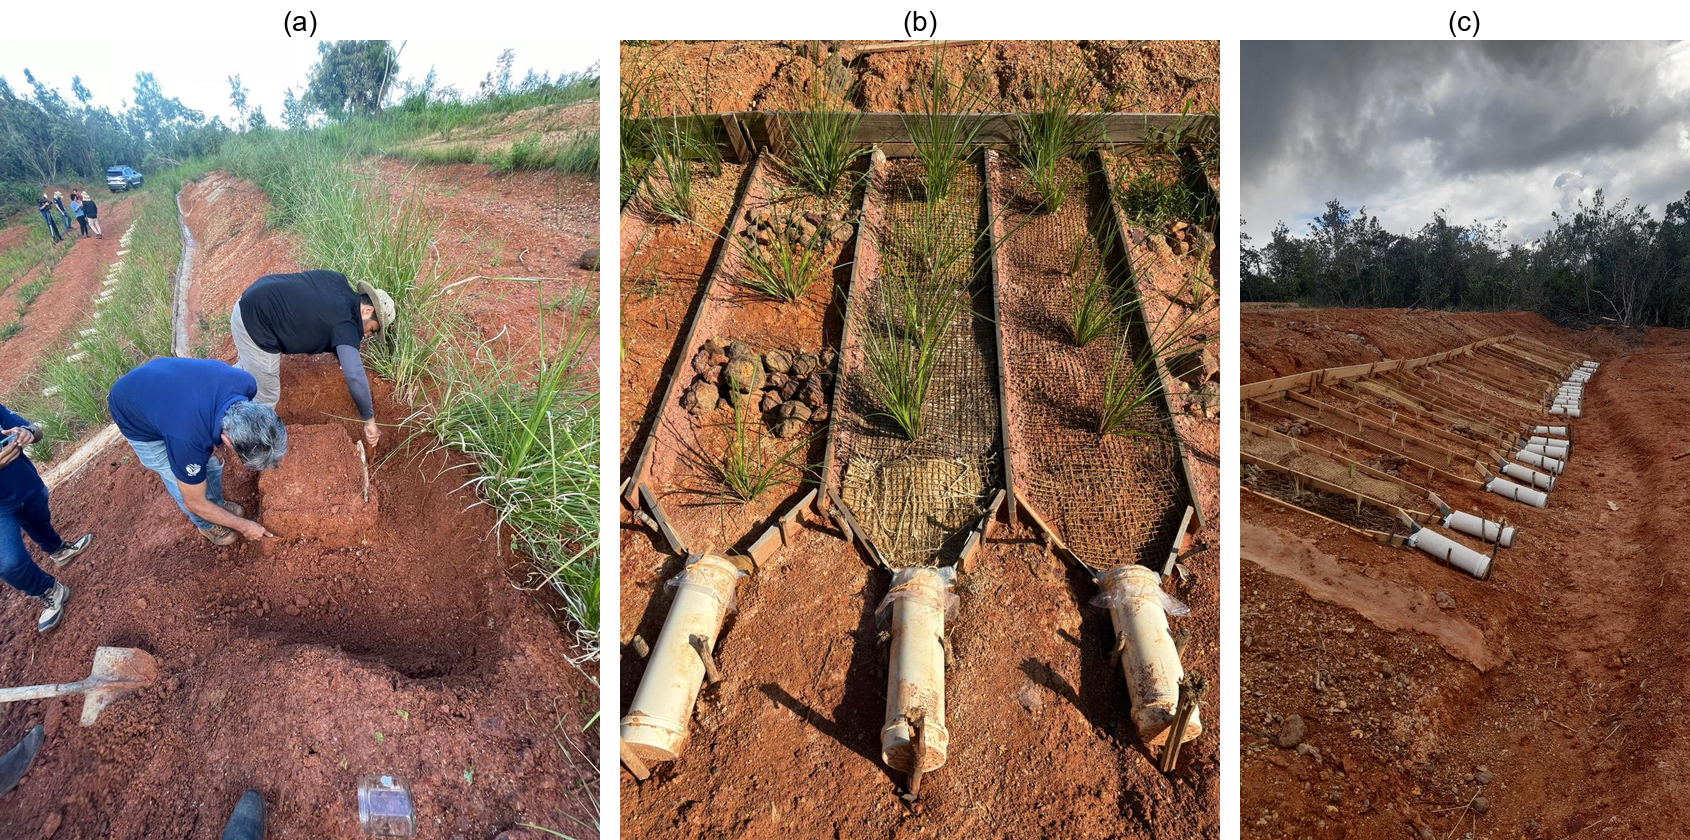
\includegraphics[width=\textwidth]{figuras/fig_09_sitio_experimental.png}
\caption{Elements of the experimental site on Haplic Plinthosol, Coastal Tablelands of Sergipe. (a)~Undisturbed block extracted for direct-shear testing ($c = 13.02$~kPa, $\phi = 34.93^\circ$). (b)~Sediment-collection plots positioned at the base of the erosion bank. (c)~General view of the bank with active erosion features. The parameters obtained from these stages directly feed the factors $\alpha$, $\beta$ and $\gamma$ of the $K_{\mathrm{plint}}$ model.}
\label{fig:sitio}
\end{figure}

\subsection{Free and fixed parameters}

The model has five free parameters ($n_1$, $\beta_{\max}$, $k_2$, $k_3$ and $n_3$) to be estimated by field calibration, and two a-priori-fixed parameters ($\mathrm{VIB_{ref}} = 6$~cm/h and $m_0 = 50\%$) derived from pedological evidence and phytotoxicity thresholds documented in tropical soils \citep{embrapa_2018}. The ratio $\delta = K_{\mathrm{plint}} / K_{\mathrm{RUSLE}} = \alpha \times \beta \times \gamma$ synthesises the total erodibility amplification and constitutes the response variable of the five computational tests described in Section~\ref{sec:validation}.

%% ================================================================
%%  3. COMPUTATIONAL VALIDATION STRATEGY
%% ================================================================
\section{Computational validation strategy}
\label{sec:validation}

\subsection{Study area and input data}

The experimental site is located in the Coastal Tablelands geomorphological unit of the state of Sergipe, northeastern Brazil, on a Haplic Plinthosol developed from sediments of the Barreiras Group \citep{nascimento_pedrotti_2004}. The climate is tropical humid (As in the K\"{o}ppen classification), with mean annual precipitation of 1200--1400~mm concentrated between April and August and mean temperature of 25~$^\circ$C. The predominant land use is degraded pasture with sparse cover, a condition that exposes the subsurface horizons to direct action of concentrated flow. The site occupies a gently undulating interfluve where the combination of sparse vegetation and subsurface plinthite has favoured the development of multiple linear erosion features along the drainage axis (Fig.~\ref{fig:area}).

\begin{figure}[htbp]
\centering
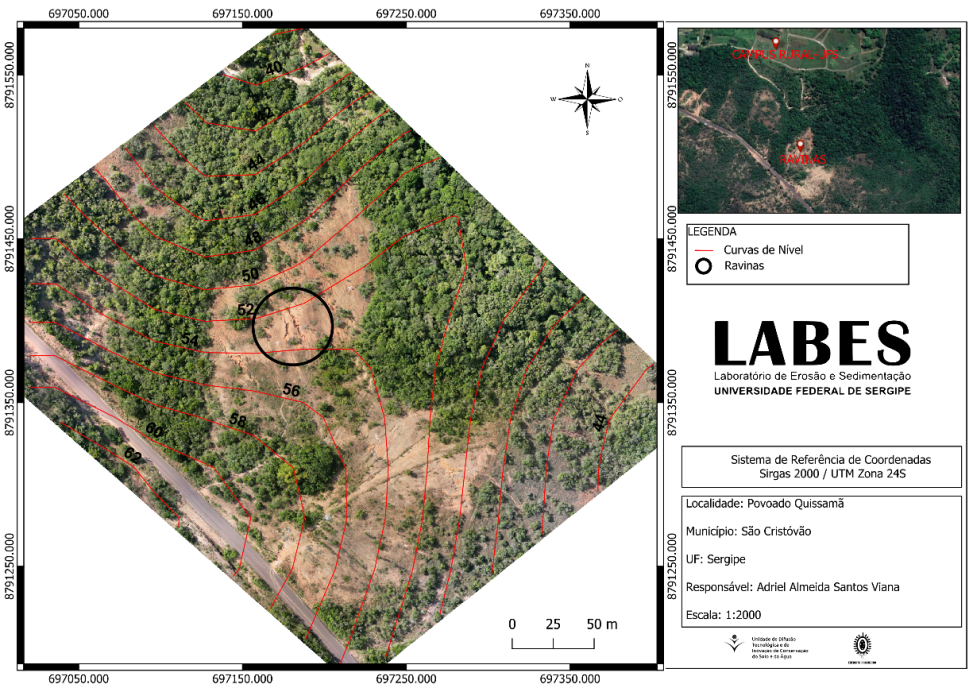
\includegraphics[width=0.85\textwidth]{figuras/fig_00a_area_estudo_aerea.png}
\caption{Aerial view of the experimental site on the Coastal Tablelands of Sergipe, northeastern Brazil, showing the degraded-pasture landscape and the occurrence of linear erosion features developed on the Haplic Plinthosol. Map lines delineate the study area and do not necessarily depict accepted national boundaries.}
\label{fig:area}
\end{figure}

Six active erosion features (F1--F6) were identified from UAV-derived orthomosaics with a mean point-cloud density of 120~points/m$^2$ and their morphometric parameters (depth, width and length) validated by direct field measurements with measuring tape (Fig.~\ref{fig:drone}). Feature depths ranged from 0.40~m (F2) to 1.50~m (F5), corresponding to normalised depths $H/H_c$ of 0.12--0.45 relative to the critical height $H_c = 3.35$~m calculated from field-measured geotechnical parameters via Eq.~\ref{eq:hc}. This interval indicates that lateral bank collapse has not yet become the dominant soil-loss mechanism in any of the surveyed features, a condition that constrains the calibration range of the geotechnical factor $\gamma$.

\begin{figure}[htbp]
\centering
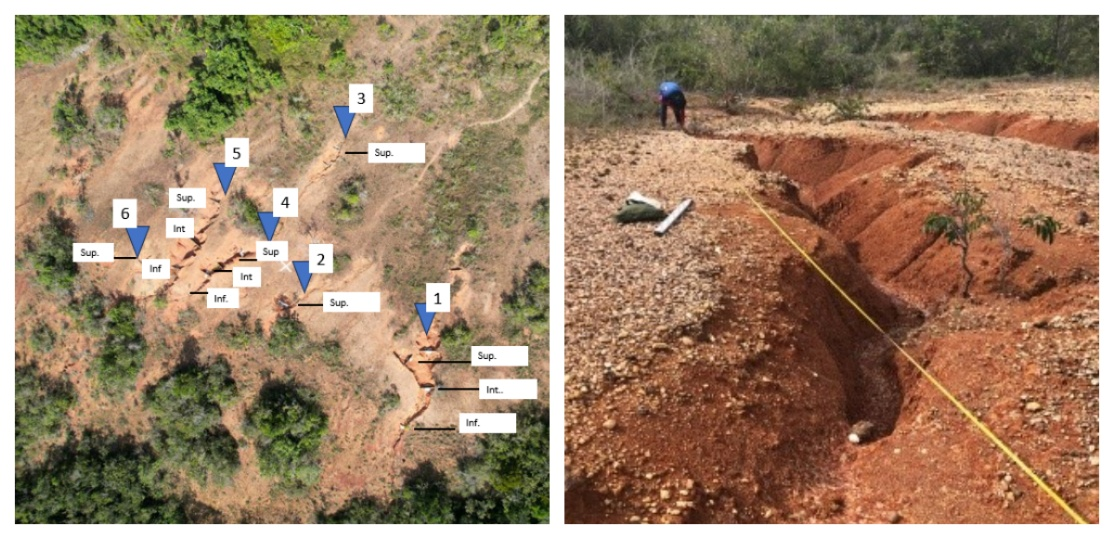
\includegraphics[width=0.85\textwidth]{figuras/fig_00b_feicoes_drone_campo.jpeg}
\caption{(a)~UAV-derived orthomosaic showing the spatial distribution of the mapped erosion features on the Haplic Plinthosol. (b)~Field measurement of morphometric parameters (depth, width and length) in one of the active erosion features.}
\label{fig:drone}
\end{figure}

All input properties of the Plinthosol were obtained from field measurements and laboratory analyses conducted on samples collected at the experimental site. The basic infiltration rate (VIB) was determined in situ by double-ring infiltrometer tests on three representative horizons (Ap, BAc and Bf), yielding values of 3.13, 1.53 and 1.59~cm/h, respectively, which confirm that the plinthic and sub-plinthic horizons impose hydraulic impedance well below the adopted reference threshold ($\mathrm{VIB_{ref}} = 6.0$~cm/h). Aluminium saturation ($m_{\mathrm{Al}}$) was quantified by routine soil-fertility analysis of samples from each genetic horizon, with values ranging from 15.2\% in the Ap to 99.2\% in the Bf, a vertical gradient consistent with progressive base leaching and exchangeable-aluminium concentration at depth. Geotechnical parameters (effective cohesion $c = 13.02$~kPa, internal friction angle $\phi = 34.93^\circ$ and saturated unit weight $\gamma_{\mathrm{sat}} = 19.93$~kN/m$^3$) were determined by direct-shear testing (ASTM D3080) on undisturbed samples extracted from the Bt horizon under saturated conditions. The erodibility $K_{\mathrm{RUSLE}} = 0.035$~t\,h\,MJ$^{-1}$\,mm$^{-1}$ was estimated from the particle-size distribution, organic-matter content, structure code and permeability class of the surface horizon using the standard nomograph \citep{wischmeier_et_al_1971}. These field-derived values constitute the primary input dataset for all five computational tests (Table~\ref{tab:profiles}, column ``Plinthosol (field)'').

Two virtual profiles (Ferralsol and Acrisol) were parameterised from median values in the regional literature for VIB, aluminium saturation, geotechnical properties and $K_{\mathrm{RUSLE}}$ \citep{silva_et_al_2009,bertoni_lombardi_neto_2017}. The Ferralsol operates as a negative control ($\alpha \approx \beta \approx \gamma \approx 1$), representing well-drained soils without hydraulic impedance, toxicity or deep erosion features, while the Acrisol functions as a partial control, sharing moderate hydraulic impedance in the Bt horizon but without plinthite or extreme aluminium toxicity. No field measurements were conducted on these two classes; their role is exclusively computational, serving as benchmarks against which the Plinthosol amplification is evaluated.

\begin{table}[htbp]
\centering
\caption{Properties of the three soil profiles used in the simulations. Plinthosol values were obtained from field measurements (double-ring infiltrometer, direct-shear testing, routine chemical and particle-size analyses); Ferralsol and Acrisol values were parameterised from regional literature.}
\label{tab:profiles}
\small
\begin{tabular}{@{}l r r r@{}}
\toprule
Property & Plinthosol (field) & Ferralsol (virtual) & Acrisol (virtual) \\
\midrule
VIB upper (cm/h) & 3.13 & 12.0 & 4.5 \\
VIB intermediate (cm/h) & 1.53 & 9.0 & 2.5 \\
VIB lower (cm/h) & 1.59 & 7.0 & 2.8 \\
$K_{\mathrm{sat,eff}}$ (cm/h) & 0.50 & 8.0 & 1.0 \\
$m_{\mathrm{Al}}$ Ap (\%) & 15.2 & 10.0 & 20.0 \\
$m_{\mathrm{Al}}$ subsurface (\%) & 84--99 & 20.0 & 45.0 \\
$c$ (kPa, saturated) & 13.02 & 30.0 & 18.0 \\
$\phi$ ($^\circ$) & 34.93 & 30.0 & 32.0 \\
$\gamma_{\mathrm{sat}}$ (kN/m$^3$) & 19.93 & 18.0 & 19.0 \\
$H_c$ (m) & 3.35 & 5.77$^a$ & 4.33$^a$ \\
$H/H_c$ mean & 0.28 & 0.00 & 0.08 \\
$K_{\mathrm{RUSLE}}$ (t\,h\,MJ$^{-1}$\,mm$^{-1}$) & 0.035 & 0.015 & 0.025 \\
\botrule
\end{tabular}
\footnotetext{$^a$ Calculated from Eq.~\ref{eq:hc}.}
\end{table}

\subsection{Target parameters for synthetic calibration}

For tests requiring known ``true'' values, the following were adopted: $n_1 = 1.0$, $\beta_{\max} = 2.5$, $k_2 = 0.10$, $k_3 = 3.0$, $n_3 = 2.0$. These values were chosen within physically plausible ranges, without claiming to represent the actual site parameters (which will only be known after field calibration).

\subsection{Test~1: Synthetic calibration (parameter recovery)}

The objective is to verify whether the proposed four-step sequential calibration protocol recovers the five known parameters from noisy data. Synthetic $\delta_{\mathrm{obs}}$ was generated for 42 virtual plots (16 Plinthosol, 12 Ferralsol, 14 Acrisol) by multiplying $\delta_{\mathrm{true}}$ by multiplicative Gaussian noise with CV of 10--30\%, so that $\delta_{\mathrm{obs}} = \delta_{\mathrm{true}} \times (1 + \varepsilon)$ with $\varepsilon \sim N(0, \mathrm{CV}^2)$, truncated at $\delta_{\mathrm{obs}} > 0$ for physical admissibility (no realisation violated this constraint in the 30 replicates). The calibration protocol follows the field sequence: negative-control verification ($\delta_{\mathrm{Lat}} \approx 1$), marginal estimation of $\alpha$ via the Acrisol, calibration of $\beta$ via the Plinthosol horizon contrast, and calibration of $\gamma$ via the geotechnical residual, followed by simultaneous optimisation via Levenberg--Marquardt. Each CV level was replicated 30 times.

\subsection{Test~2: Global sensitivity analysis (Sobol)}

First-order ($S_1$) and total ($S_T$) Sobol indices \citep{sobol_2001} were calculated to quantify each parameter's contribution to the variance of $\delta$ in four representative scenarios: Plinthosol intermediate (VIB = 1.53, $m = 84\%$, $H/H_c = 0.33$), Plinthosol upper (VIB = 3.13, $m = 15\%$, $H/H_c = 0.12$), Acrisol (VIB = 2.5, $m = 45\%$, $H/H_c = 0.08$) and Ferralsol (VIB = 9.0, $m = 20\%$, $H/H_c = 0$). Saltelli sampling \citep{saltelli_et_al_2004} with $N = 1024$ generated 12\,288 model evaluations. The five parameters were sampled as independent uniform variables, a premise supported by the multiplicative formulation in which $\alpha$, $\beta$ and $\gamma$ represent physically distinct mechanisms without a-priori parametric correlation. Parameter bounds were $n_1 \in [0.1, 3.0]$, $\beta_{\max} \in [1.1, 5.0]$, $k_2 \in [0.01, 0.50]$, $k_3 \in [0.5, 10.0]$ and $n_3 \in [1.0, 4.0]$.

\subsection{Test~3: Slope stability and \texorpdfstring{$\gamma$}{gamma} validation}
\label{sec:test3}

The Rankine factor of safety (FS) \citep{rankine_1857} for vertical cuts was calculated for $H/H_c$ from 0.05 to 0.95 under six levels of relative pore pressure ($r_u = 0$ to 0.5), using the field geotechnical parameters of the Plinthosol. The volume mobilised by a planar failure wedge was normalised and modelled as a geotechnical contribution proxy ($\delta_{\mathrm{geo}} \propto V_{\mathrm{norm}}/\mathrm{FS}$). The function $\gamma = 1 + k_3(H/H_c)^{n_3}$ was fitted to the proxy by non-linear least squares, and the FS corresponding to each of the six real features (F1--F6) was verified.

\subsection{Test~4: Infiltration and runoff generation (Green--Ampt)}

A Green--Ampt infiltration model \citep{green_ampt_1911} was applied to the three soil profiles under rainfall events with $I_{30}$ of 5--100~mm/h and duration of 60~min. The effective $K_{\mathrm{sat}}$ of each profile corresponds to the limiting horizon (minimum across layers). The runoff coefficient (CE) was calculated and the ratio $\mathrm{CE}_{\mathrm{soil}}/\mathrm{CE}_{\mathrm{Ferralsol}}$ compared with $\alpha(\mathrm{VIB})$ for different values of $n_1$, evaluating the consistency between the analytical hydraulic model and the proposed functional form.

\subsection{Test~5: Virtual erosion (simplified WEPP-type model)}

The runoff generated by the Green--Ampt model was converted to bed shear stress ($\tau = \rho g h S$, uniform Manning regime) and to soil loss via a detachment model ($D = k_r(\tau - \tau_c)$ for $\tau > \tau_c$). The erodibility $K_{\mathrm{obs}}$ was inverted via the USLE relationship ($K_{\mathrm{obs}} = A/(EI_{30} \times LS)$) and the discrepancy $\delta_{\mathrm{obs}} = K_{\mathrm{obs}}/K_{\mathrm{RUSLE}}$ compared with $\delta_{\mathrm{mod}}$ predicted by Eq.~\ref{eq:kplint} using the target parameters of Section~3.2. Intrinsic erodibility parameters ($k_r$, $\tau_c$) were estimated from the literature for tropical soils.

%% ================================================================
%%  4. RESULTS AND DISCUSSION
%% ================================================================
\section{Results and Discussion}
\label{sec:results}

\subsection{Parameter recovery (Test~1)}

The sequential calibration protocol recovered the three hydraulic-biological parameters ($n_1$, $\beta_{\max}$, $k_2$) with median relative bias below 15\% for all noise levels tested (Fig.~\ref{fig:calibracao}), with precision decreasing in the order $n_1 > k_2 > \beta_{\max}$ under CV of 30\%. The greater recoverability of $n_1$ (median 1.01--1.18 versus the true value of 1.0) is coherent with the dominance of the hydraulic term in the variance of $\delta$ in the Plinthosol and has direct implications for field calibration, since residual errors in this exponent propagate multiplicatively to the soil-loss estimate. The maximum toxicity amplification ($\beta_{\max} = 2.28$--2.85, true 2.5) and the transition rate ($k_2 = 0.11$--0.13, true 0.10) exhibited comparable biases whose propagation is attenuated by the narrower range of $m_{\mathrm{Al}}$ in the horizons exposed at gully banks, although the dispersion of $\beta_{\max}$ increased with noise level without generating a systematic trend.

\begin{figure}[htbp]
\centering

\includegraphics[width=0.9\textwidth]{figuras/fig_01_calibracao_sintetica.png}
\caption{Median relative bias of estimated parameters as a function of the coefficient of variation (CV) of noise applied to synthetic data. The four-step sequential protocol followed by simultaneous Levenberg--Marquardt optimisation recovers the hydraulic exponent ($n_1$), the maximum toxicity amplification ($\beta_{\max}$) and the sigmoid transition rate ($k_2$) with bias below 15\% for CV up to 30\%. The geotechnical parameters ($k_3$ and $n_3$) exhibit equifinality (bias $>$\,50\%) due to low individual sensitivity in the normalised depth interval $H/H_c = 0.12$--0.45.}
\label{fig:calibracao}
\end{figure}

The parameters $k_3$ and $n_3$ exhibited high dispersion and a tendency to converge at the upper bounds of the search ranges (Fig.~\ref{fig:boxplot}), with medians of $k_3$ reaching 14.9 and $n_3$ reaching 3.9 for CV = 30\% (true values 3.0 and 2.0). This instability is expected because, for $H/H_c = 0.12$--0.45 (the range of real features), the product $k_3 \times (H/H_c)^{n_3}$ admits multiple combinations with $\gamma$ near~1.0, generating equifinality between $k_3$ and $n_3$. The phenomenon is analogous to that described by \citet{beven_freer_2001} for mechanistic hydrological models, in which distinct parameter sets produce equally acceptable responses within observational uncertainty bounds, and by \citet{beven_2006}, who formalised equifinality as an intrinsic property of over-parameterised models relative to available information. \citet{her_chaubey_2015} demonstrated that equifinality tends to diminish as the number of observations increases and the temporal distribution of data covers the model's dynamic range, a finding that, transposed to the present context, indicates that incorporating features with $H/H_c > 0.45$ may reduce the indeterminacy of $k_3$ and $n_3$ by forcing the model to differentiate trajectories that, in the current interval, remain collinear.

Since the field data from the Plinthosol lack features with $H/H_c > 0.45$, the range where $\gamma$ would differentiate more markedly, calibration of this factor requires monitoring of features with depth exceeding 1.5~m ($H/H_c > 0.45$) or complementary geotechnical modelling to constrain the search space, as corroborated by the slope-stability analysis with the Rankine model.

\begin{figure}[htbp]
\centering

\includegraphics[width=\textwidth]{figuras/fig_02_boxplot_parametros.png}
\caption{Distribution of estimated parameters across 30 replicates per noise level. Red dashed lines indicate the true values. The hydraulic exponent ($n_1$), maximum toxicity amplification ($\beta_{\max}$) and sigmoid transition rate ($k_2$) remain centred on the true values, whereas the scale ($k_3$) and curvature ($n_3$) of the geotechnical factor show increasing dispersion with equifinality.}
\label{fig:boxplot}
\end{figure}

The negative control (Ferralsol) yielded a median $\delta_{\mathrm{Lat}}$ of 1.04--1.07 across all CV levels, confirming that the model correctly predicts $\delta \approx 1$ when the three amplifying conditions are absent. This behaviour is expected from the multiplicative formulation, in which $\alpha = 1$ for $\mathrm{VIB} \geq \mathrm{VIB_{ref}}$, $\beta \approx 1$ for $m_{\mathrm{Al}} < 50\%$ and $\gamma = 1$ for $H/H_c = 0$, so that any residual noise in the Ferralsol $\delta$ is attributable solely to the numerical propagation of parameter uncertainty and not to a structural model tendency. The proximity of $\delta_{\mathrm{Lat}}$ to unity across all realisations reinforces the pedological specificity of the correction factor and is coherent with the finding that deep Ferralsols tend to exhibit plot-measured erodibility near or below the nomograph estimate, owing to the stable macroaggregation promoted by iron and aluminium oxides that the nomograph does not incorporate \citep{cassol_et_al_2023}. \citet{auerswald_et_al_2014} demonstrated that the original nomograph equation overestimates $K$ in soils with stable aggregates and high hydraulic conductivity --- a typical Ferralsol condition --- whereas \citet{ostovari_et_al_2016} observed underestimation in calcareous soils with subsurface hydraulic impedance, a pattern analogous to that of Plinthosols. This asymmetry of nomograph error across pedological classes indicates that the experimental design with a negative control is indispensable for isolating the effects of each amplifier during field calibration, since only comparison with a soil where $\delta \approx 1$ permits attribution of discrepancies observed in the Plinthosol to the subsurface mechanisms represented by the correction factor with greater confidence.

\subsection{Sensitivity hierarchy (Test~2)}

Identification of the most influential parameter before field calibration is a necessary condition for efficiently allocating instrumental effort, since parameters with low sensitivity may be fixed by independent evidence without predictive loss \citep{saltelli_et_al_2004}. \citet{chaves_nearing_1991} demonstrated, in an uncertainty analysis of the WEPP model, that interrill erodibility and hydraulic conductivity accounted for more than 70\% of the variance in predicted soil loss, while roughness and cover parameters contributed secondarily, a pattern that anticipates the hierarchy observed here between the hydraulic mechanism and the remaining factors. In the present model, Sobol analysis revealed that $n_1$ governs 63\% of the variance of $\delta$ for the intermediate Plinthosol scenario ($\mathrm{VIB} = 1.53$~cm/h, $m = 84\%$, $H/H_c = 0.33$), with $S_T = 0.84$ indicating relevant interactions with $\beta_{\max}$ and $n_3$ (Fig.~\ref{fig:sobol}). In the upper Plinthosol scenario ($\mathrm{VIB} = 3.13$~cm/h), $n_1$ dominates even more markedly ($S_1 = 0.78$, $S_T = 0.85$) because the smaller VIB/$\mathrm{VIB_{ref}}$ gradient reduces the relative sensitivity of the remaining terms.

\begin{figure}[htbp]
\centering

\includegraphics[width=\textwidth]{figuras/fig_03_sensibilidade_sobol.png}
\caption{Sobol first-order ($S_1$) and total ($S_T$) sensitivity indices for four representative scenarios. The hydraulic exponent ($n_1$) dominates the amplification factor ($\delta$) variance for the Plinthosol and Acrisol, whereas the toxicity sigmoid transition rate ($k_2$) dominates for the Ferralsol, whose basic infiltration rate exceeds the reference threshold ($\mathrm{VIB_{ref}} = 6$~cm/h), nullifying the hydraulic factor ($\alpha = 1$) and concentrating variance in the toxicity factor ($\beta$).}
\label{fig:sobol}
\end{figure}

The Acrisol exhibited a pattern similar to the Plinthosol ($S_1$ of $n_1 = 0.79$), indicating that in soils with $\mathrm{VIB} < \mathrm{VIB_{ref}}$ the hydraulic regime is the dominant mechanism in the amplification of $\delta$, a result consistent with the expectation that subsurface impedance governs the largest share of variance in this profile, whereas the Ferralsol, operating with $\mathrm{VIB} > \mathrm{VIB_{ref}}$ (hence $\alpha = 1$), transfers the variance to $k_2$ ($S_1 = 0.70$, $S_T = 0.93$), the parameter governing the toxicity sigmoid transition. The concordance between parametric hierarchy and expected pedological mechanism indicates internal consistency of the model and that the multi-class design is necessary for balanced calibration of the five parameters. The dominance of the hydraulic mechanism over total variance is consistent with the findings of \citet{francois_et_al_2024}, who identified the $K$ factor as the most sensitive parameter in RUSLE applied to southern Bahia, and with the proposition of \citet{alewell_et_al_2019} that the nomograph transferability to tropical environments is limited by the absence of representation of subsurface processes. In Mediterranean contexts, \citet{bagarello_et_al_2012} observed that plot-measured erodibility in southern Italy systematically exceeded nomograph estimates in soils with a subsurface clay horizon, reinforcing the indication that hydraulic impedance from textural discontinuity is a recognised $K$ amplifier across different geomorphological provinces, although the underlying mechanism in tropical Plinthosols additionally involves iron-oxide cementation absent in Mediterranean soils.

The second-order interaction matrix ($S_2$) for the intermediate Plinthosol (Fig.~\ref{fig:interacoes}) indicated relevant interaction between $n_1$ and $\beta_{\max}$ ($S_2 \approx 0.05$--0.10) and between $k_3$ and $n_3$ ($S_2 \approx 0.02$), corroborating the equifinality between $k_3$ and $n_3$ identified in the synthetic calibration and suggesting that constraining $n_3$ via geotechnical modelling may decouple this interaction. The interaction between $n_1$ and $\beta_{\max}$ has a direct physical interpretation, since in profiles with low VIB and high $m_{\mathrm{Al}}$ both amplifying terms operate simultaneously, and the magnitude of the product $\alpha \times \beta$ depends on the non-linear combination of their exponents, whereas the $k_3$--$n_3$ interaction is purely parametric and arises from the flattened response surface of $\gamma$ in the interval $H/H_c < 0.45$. The distinction between mechanistic interactions and spurious indeterminacy interactions is relevant for field-experimental planning, since the former demands plots that capture the real covariance between infiltration and toxicity, while the latter may be mitigated by prior constraint of the parameter space via independent geotechnical modelling.

\begin{figure}[htbp]
\centering
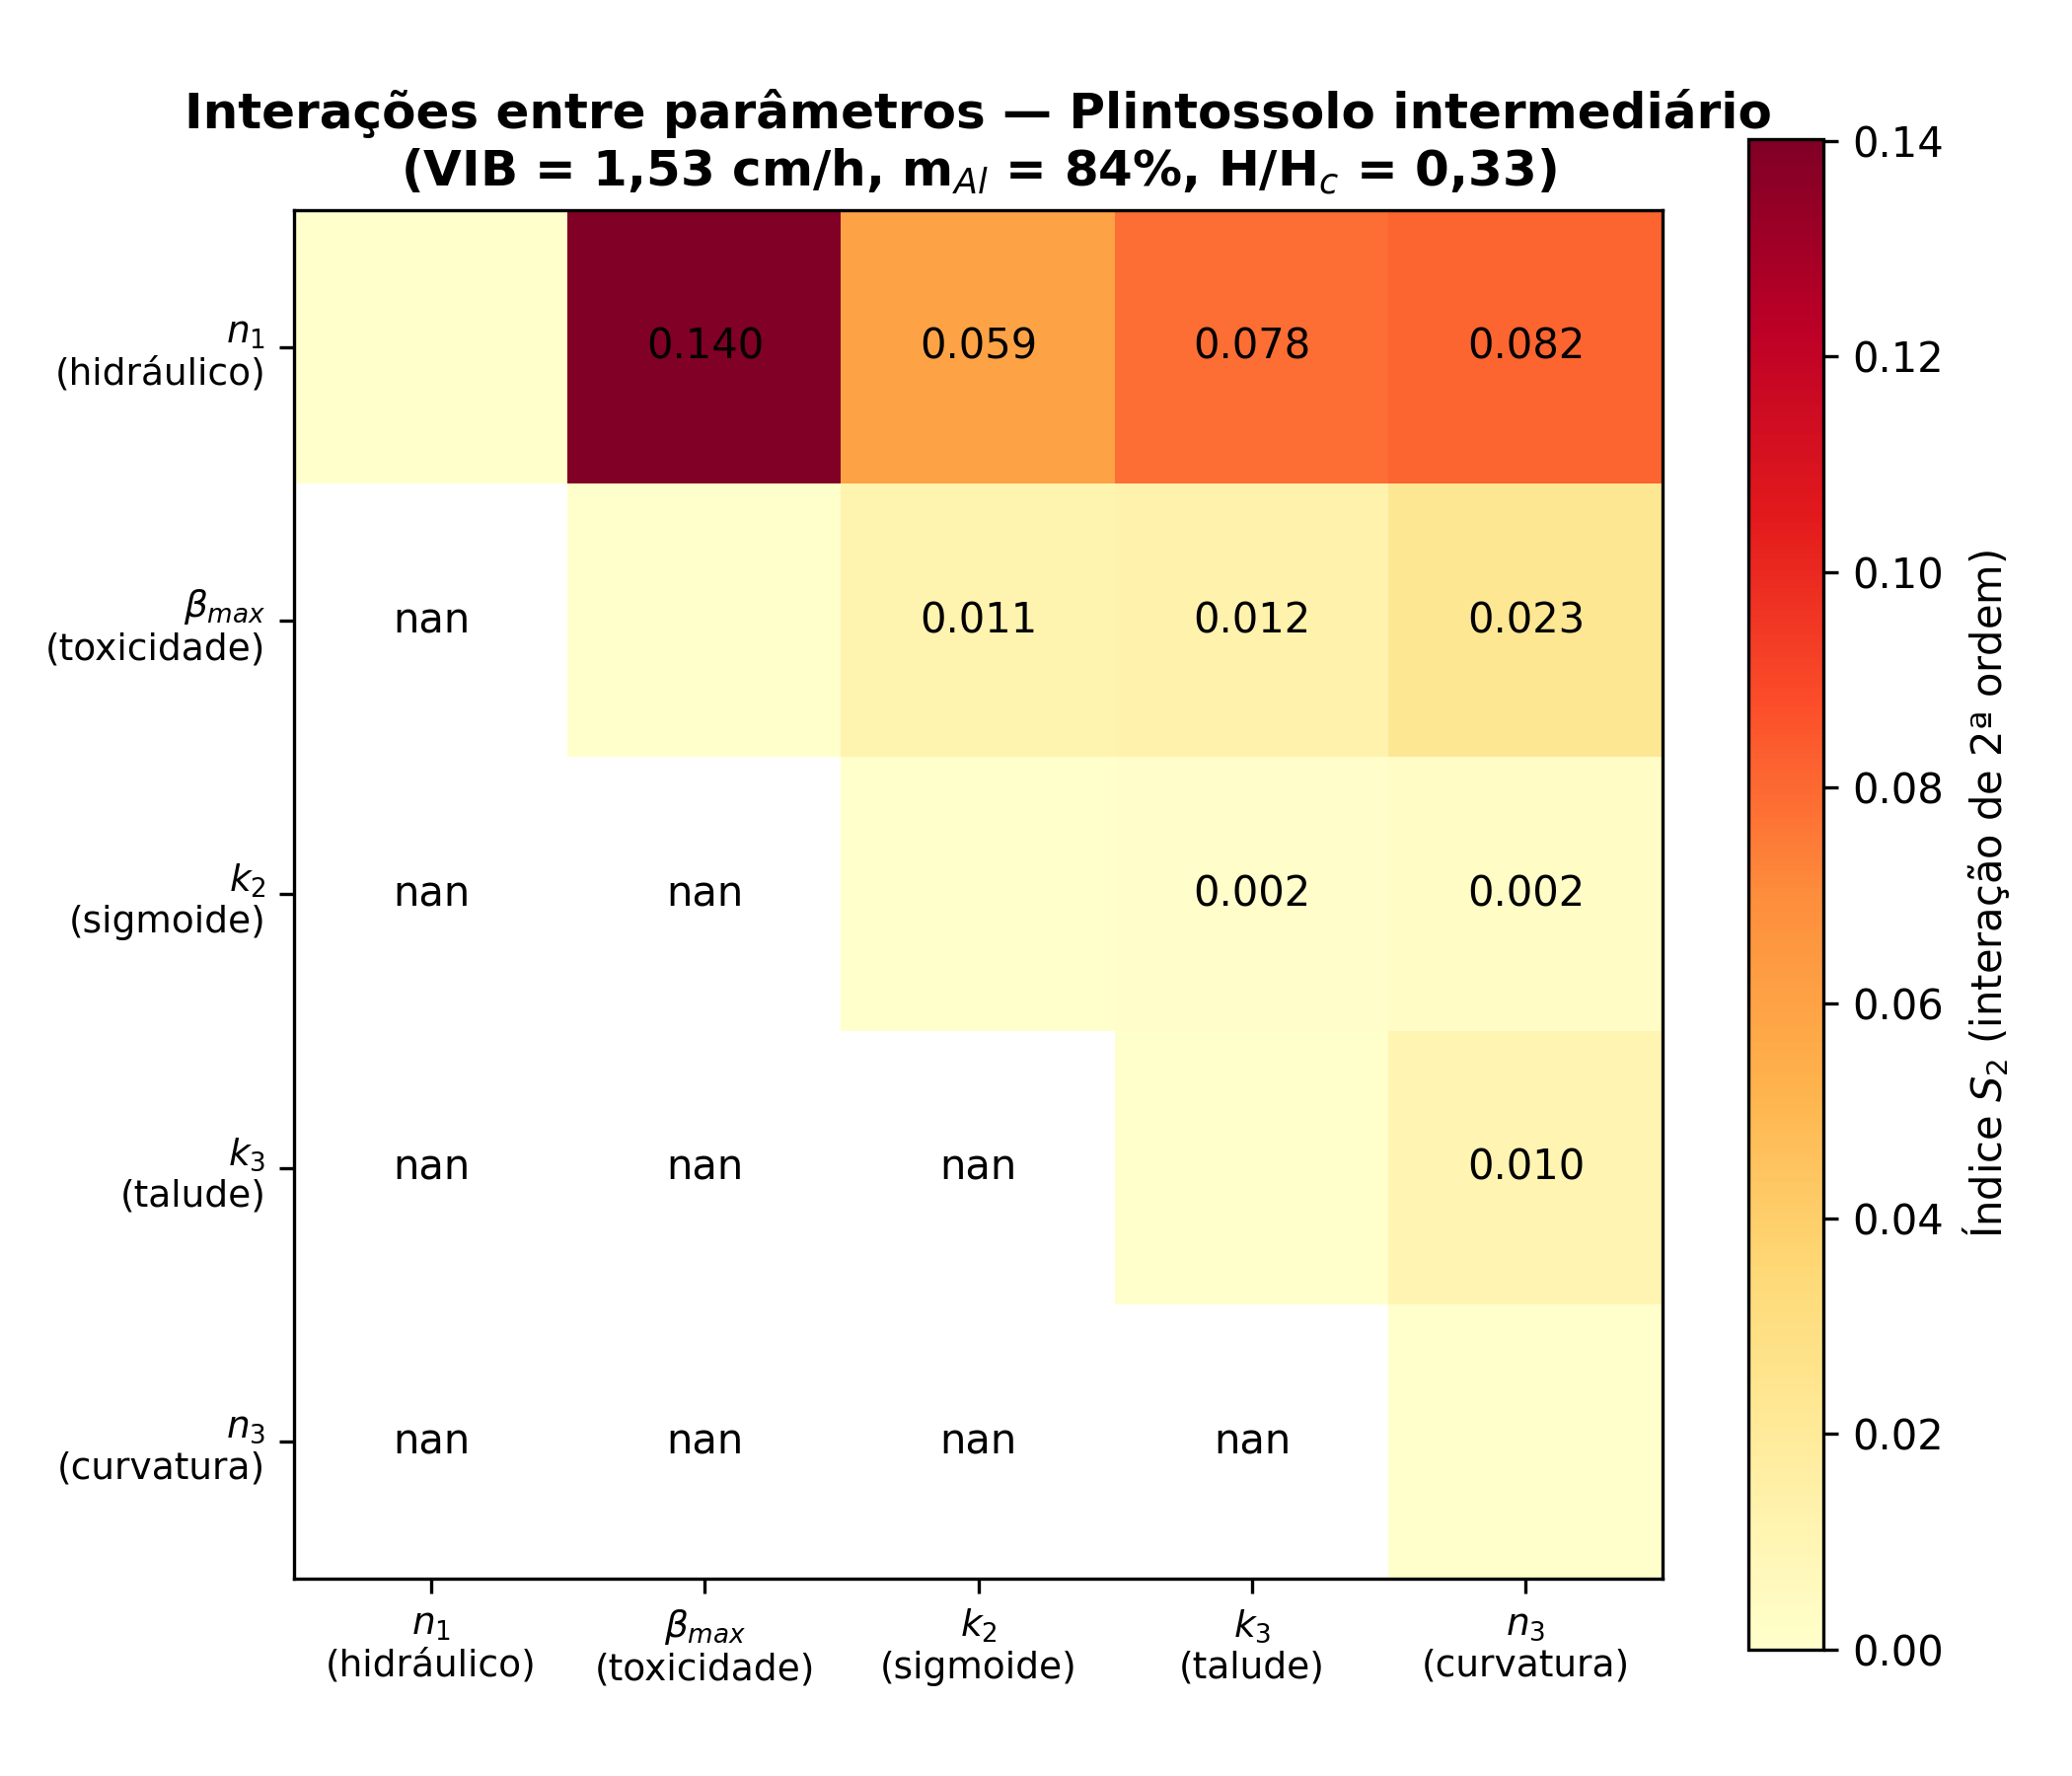
\includegraphics[width=0.7\textwidth]{figuras/fig_04_interacoes_s2.png}
\caption{Sobol second-order interaction matrix ($S_2$) for the intermediate Plinthosol scenario ($\mathrm{VIB} = 1.53$~cm/h, aluminium saturation $= 84\%$, $H/H_c = 0.33$). Values of $S_2$ exceeding 0.05 indicate parametric interactions that field calibration must resolve simultaneously.}
\label{fig:interacoes}
\end{figure}

\subsection{Geotechnical validation of \texorpdfstring{$\gamma$}{gamma} (Test~3)}

The fit of $\gamma = 1 + k_3(H/H_c)^{n_3}$ to the geotechnical contribution proxy ($\delta_{\mathrm{geo}}$) derived from the Rankine model converged to $k_3 = 6.50$ and $n_3 = 4.51$ (Fig.~\ref{fig:taludes}), values substantially higher than the synthetic-calibration target parameters ($k_3 = 3.0$, $n_3 = 2.0$). This divergence is physically coherent because the volumetric contribution of collapse grows more rapidly with $H/H_c$ than the originally proposed quadratic expansion, owing to the cubic or quartic dependence of wedge volume on wall height \citep{fredlund_rahardjo_1993}. The exponent $n_3 \approx 4.5$ suggests that the geotechnical contribution remains negligible for $H/H_c < 0.3$ and rises abruptly above this threshold, consistent with the field observation that only F4 ($H/H_c = 0.42$) and F5 (0.45) were classified as incipient gullies by the fuzzy system. \citet{oliveira_1991}  observed analogous behaviour in gullies developed on Barreiras Group sediments in Bananal (SP), where bank geometry conditioned the transition between concentrated-flow erosion and mass failure, with significant collapses occurring only when the depth-to-width ratio exceeded a geometric threshold equivalent to $H/H_c \approx 0.35$--0.40 under those site conditions. \citet{vandekerckhove_et_al_2003} quantified headcut retreat rates in southeastern Spain at 0.01--0.89~m/yr using multi-temporal aerial photographs, finding that the highest rates were associated with features having vertical walls and depth exceeding 1.5~m, a condition in which gravitational instability surpasses hydraulic detachment as the dominant mechanism of feature advance. \citet{campo_bescos_et_al_2013} corroborated this relationship by validating a headcut-retreat model calibrated with multi-temporal digital elevation models, in which the geotechnical lateral-collapse component exceeded the hydraulic base-scouring component for high $H/H_c$ ratios, a pattern supporting the pronounced non-linearity ($n_3 > 4$) observed in the present fit.

\begin{figure}[htbp]
\centering
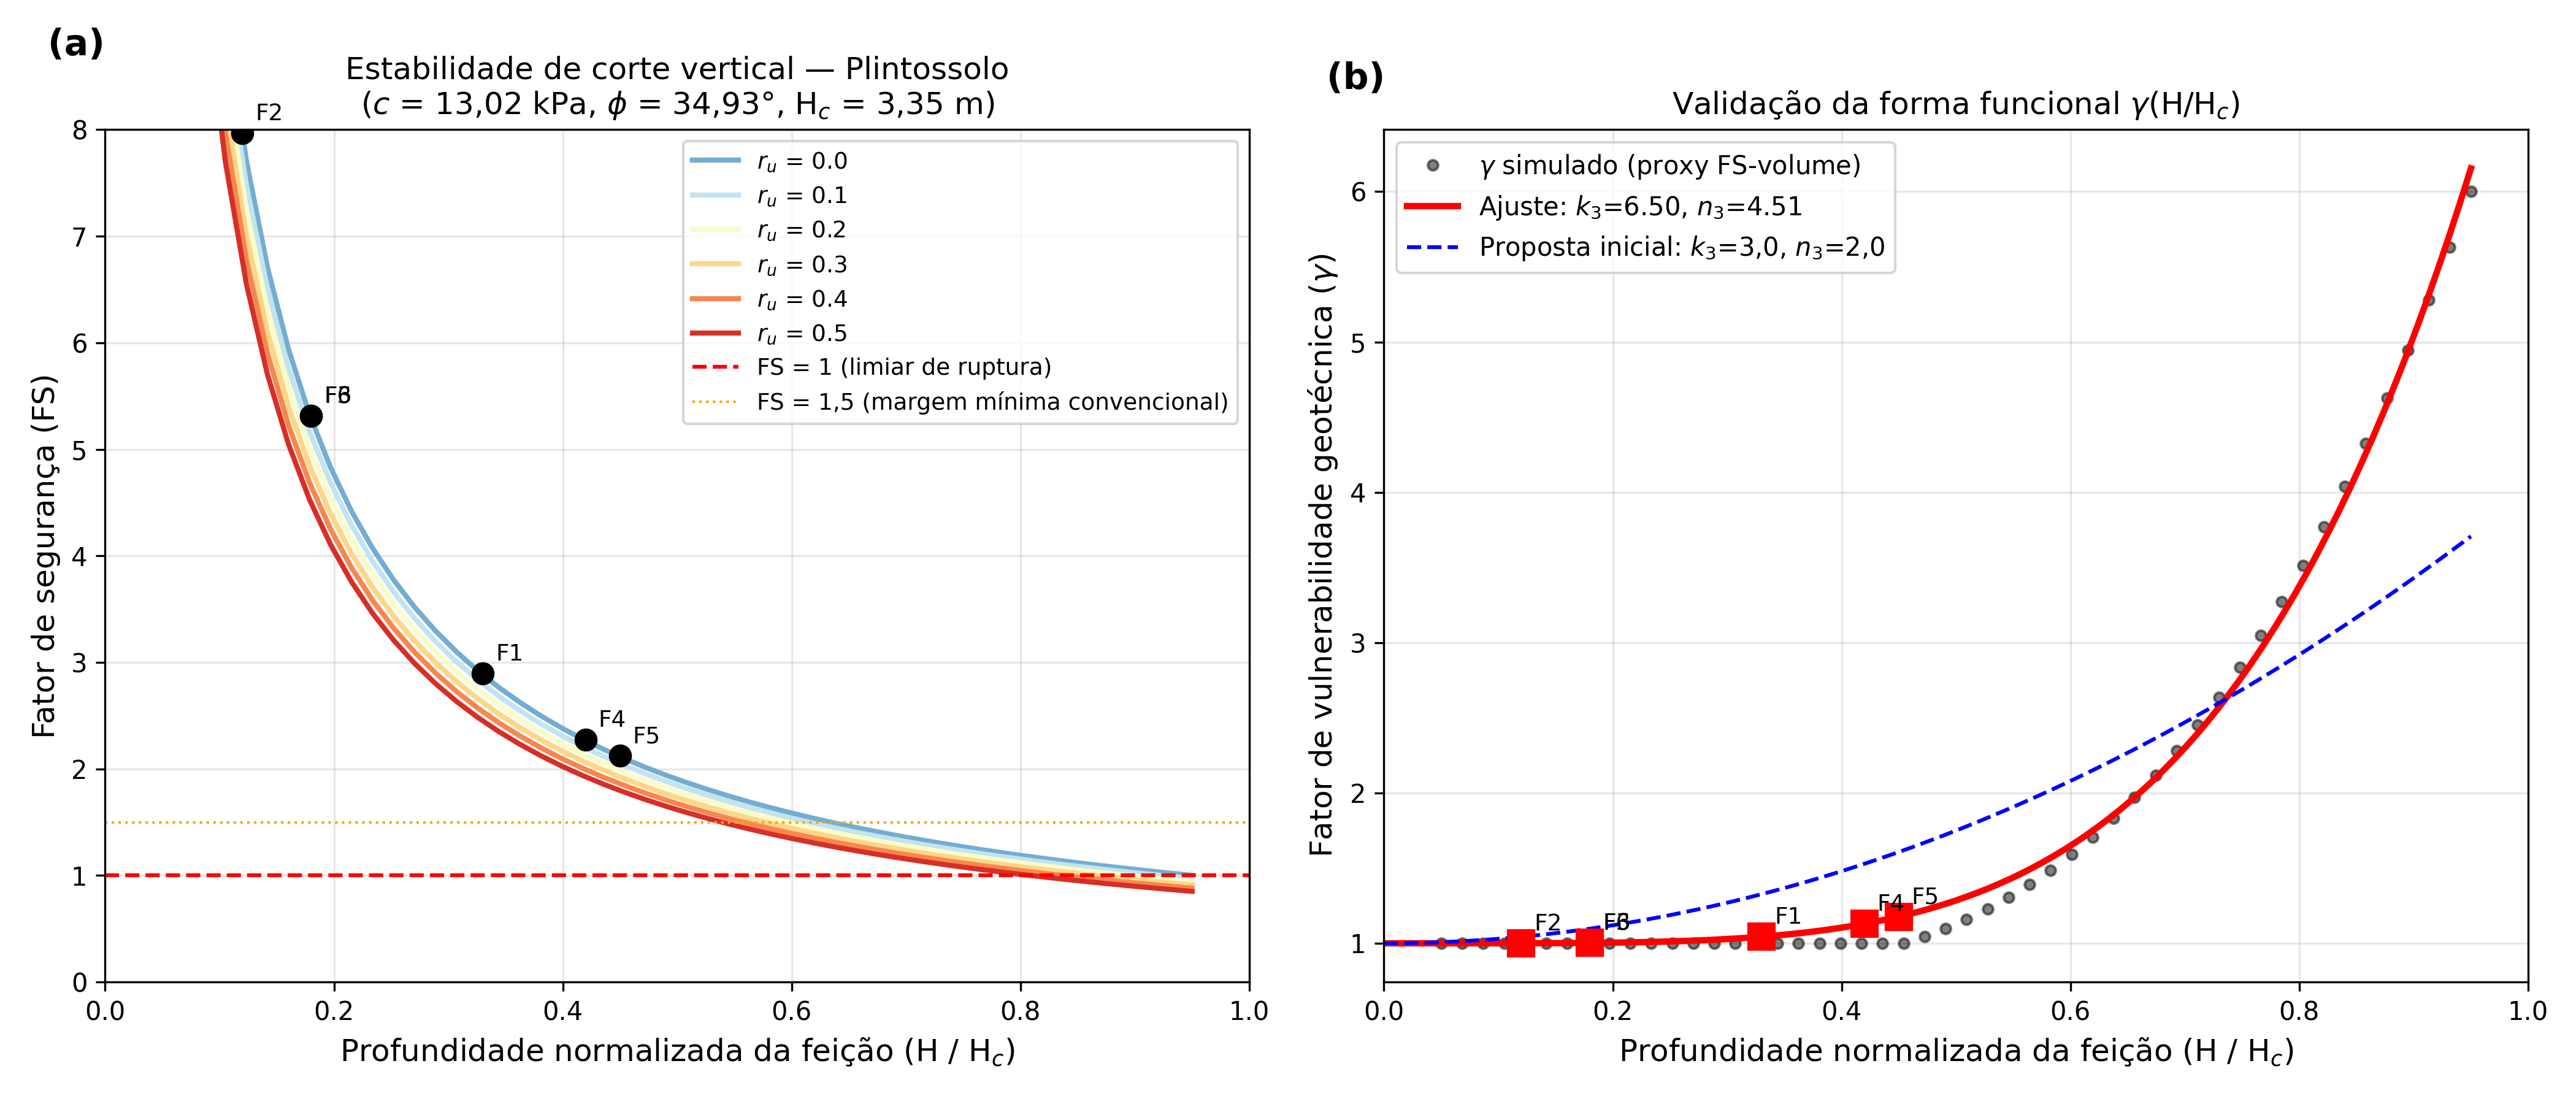
\includegraphics[width=\textwidth]{figuras/fig_05_estabilidade_taludes.png}
\caption{Geotechnical validation of the bank-vulnerability factor ($\gamma$). (a)~Rankine factor of safety (FS) for vertical cuts as a function of normalised feature depth ($H/H_c$, ratio between actual depth and critical collapse height) under different relative pore pressures ($r_u$). (b)~Geotechnical contribution proxy ($\delta_{\mathrm{geo}}$) and power fit $\gamma = 1 + 6.50 \times (H/H_c)^{4.51}$. Red dots indicate the six real erosion features (F1--F6), all with FS $>$\,1 under current conditions.}
\label{fig:taludes}
\end{figure}

The sensitivity of FS to relative pore pressure ($r_u$) is relevant for stability prognosis, since FS values decrease from 2.12 to 1.93 in F5 when $r_u$ increases from 0 to 0.3, and under prolonged saturation during extreme rainfall events this reduction may bring FS close to unity and trigger lateral collapses that feedback soil loss via geotechnical pathways, a mechanism that \citet{vanmaercke_et_al_2021} identified as responsible for up to 60\% of volumetric gully advance in subtropical regions.

All six real features exhibited FS $>$\,2.0 for $r_u = 0$ and FS $>$\,1.8 for $r_u = 0.3$ (Table~\ref{tab:fs}), indicating a geotechnical safety margin consistent with classification as gullies without active collapse according to the criteria of \citet{poesen_2018}, for whom the distinction between rill and gully is conditioned by the depth sufficient to mobilise soil volumes by gravitational failure.

The fitted $\gamma$ for F5 ($H/H_c = 0.45$) reached 1.18, indicating 18\% geotechnical amplification over the basal erodibility, while F2 ($H/H_c = 0.12$) remains at $\gamma = 1.00$. This differentiation sustains the expectation of pronounced non-linearity of the geotechnical contribution and suggests that, for features with $H/H_c > 0.6$ (not observed at this site but documented in regional gullies), $\gamma$ may exceed~2.0, a condition in which the geotechnical mechanism would contribute with magnitude comparable to or exceeding the hydraulic and phytotoxic amplification.

\begin{table}[htbp]
\centering
\caption{Factor of safety and fitted $\gamma$ for the six real erosion features.}
\label{tab:fs}
\small
\begin{tabular}{@{}c r r r r r@{}}
\toprule
Feature & $H$ (m) & $H/H_c$ & FS ($r_u = 0$) & FS ($r_u = 0.3$) & $\gamma$ fitted \\
\midrule
F1 & 1.10 & 0.33 & 2.90 & 2.64 & 1.04 \\
F2 & 0.40 & 0.12 & 7.97 & 7.25 & 1.00 \\
F3 & 0.60 & 0.18 & 5.31 & 4.83 & 1.00 \\
F4 & 1.40 & 0.42 & 2.28 & 2.07 & 1.13 \\
F5 & 1.50 & 0.45 & 2.12 & 1.93 & 1.18 \\
F6 & 0.60 & 0.18 & 5.31 & 4.83 & 1.00 \\
\botrule
\end{tabular}
\end{table}

\subsection{Runoff generation and \texorpdfstring{$\alpha$}{alpha} validation (Test~4)}

The adoption of the limiting-horizon $K_{\mathrm{sat}}$ as $K_{\mathrm{sat,eff}}$ follows the formulation of \citet{wang_et_al_1999} for infiltration in stratified soils, in which the least-permeable layer controls the time to ponding and accumulated runoff volume independently of the upper-layer conductivity. This premise is particularly suitable for profiles with a plinthic horizon whose conductivity is one to two orders of magnitude below that of the overlying A horizon.

The Green--Ampt infiltration model confirmed the hydrological differentiation among the three classes (Fig.~\ref{fig:infiltracao}a). The Plinthosol ($K_{\mathrm{sat,eff}} = 0.50$~cm/h, limiting BAc horizon) generated a runoff coefficient of 0.20 for $I_{30} = 30$~mm/h and 0.56 for $I_{30} = 60$~mm/h, reflecting the subsurface hydraulic impedance that converts the non-infiltrated precipitation fraction to Hortonian runoff even under moderate intensities. The Acrisol ($K_{\mathrm{sat,eff}} = 1.0$~cm/h) yielded CE = 0.37 for $I_{30} = 60$~mm/h, intermediate between the two extremes and consistent with the partial impedance of the plinthite-free Bt horizon.

\begin{figure}[htbp]
\centering

\includegraphics[width=\textwidth]{figuras/fig_06_infiltracao_escoamento.png}
\caption{(a)~Runoff coefficient (CE) as a function of maximum 30-minute intensity ($I_{30}$) for the three soil profiles simulated by the Green--Ampt infiltration model (60-min event). (b)~Ratio between each soil's CE and the Ferralsol CE compared with the theoretical hydraulic amplification factor ($\alpha$) from Eq.~\ref{eq:alpha} for three values of the exponent $n_1$. The Ferralsol generates no surface runoff at any tested intensity, consistent with $\alpha = 1$ for the negative control.}
\label{fig:infiltracao}
\end{figure}

The Ferralsol ($K_{\mathrm{sat,eff}} = 8.0$~cm/h) generated no surface runoff at any of the tested intensities (CE = 0 for $I_{30}$ up to 100~mm/h), indicating that the threshold $\mathrm{VIB_{ref}} = 6$~cm/h is conservative and that soils with effective $K_{\mathrm{sat}}$ exceeding this level tend to operate fully in an infiltration-dominated regime. The runoff coefficient of 0.56 obtained for the Plinthosol under $I_{30} = 60$~mm/h is compatible with the runoff magnitude expected in soils whose limiting horizon has $K_{\mathrm{sat}}$ below 1~cm/h \citep{morgan_2005}, while the absence of runoff in the Ferralsol is coherent with the hydrological behaviour of deep, well-drained soils \citep{bertoni_lombardi_neto_2017}. This condition validates the formulation of $\alpha$ (Eq.~\ref{eq:alpha}), in which $\alpha = 1$ for $\mathrm{VIB_{local}} \geq \mathrm{VIB_{ref}}$, and supports the use of the Ferralsol as a genuine negative control where $K_{\mathrm{obs}} \approx K_{\mathrm{RUSLE}}$.

The runoff hydrograph under $I_{30} = 60$~mm/h (Fig.~\ref{fig:hidrograma}) illustrates the temporal difference in runoff generation, with the Plinthosol reaching steady state in less than 10~min while the Acrisol requires approximately 25~min, a difference reflecting the inverse proportion between $K_{\mathrm{sat,eff}}$ and the time to ponding predicted by infiltration-excess theory \citep{horton_1933}. The absence of Ferralsol runoff throughout the 60-min event is coherent with soils whose effective $K_{\mathrm{sat}}$ exceeds any probable rainfall intensity at the study site. The temporal contrast between Plinthosol and Acrisol may have implications for the dimensioning of erosion-control structures, since the earlier onset of peak runoff in soils with plinthic horizons suggests that erosive energy reaches high values before dissipative interventions such as permeable check-dams can accumulate upstream sediment.

\begin{figure}[htbp]
\centering
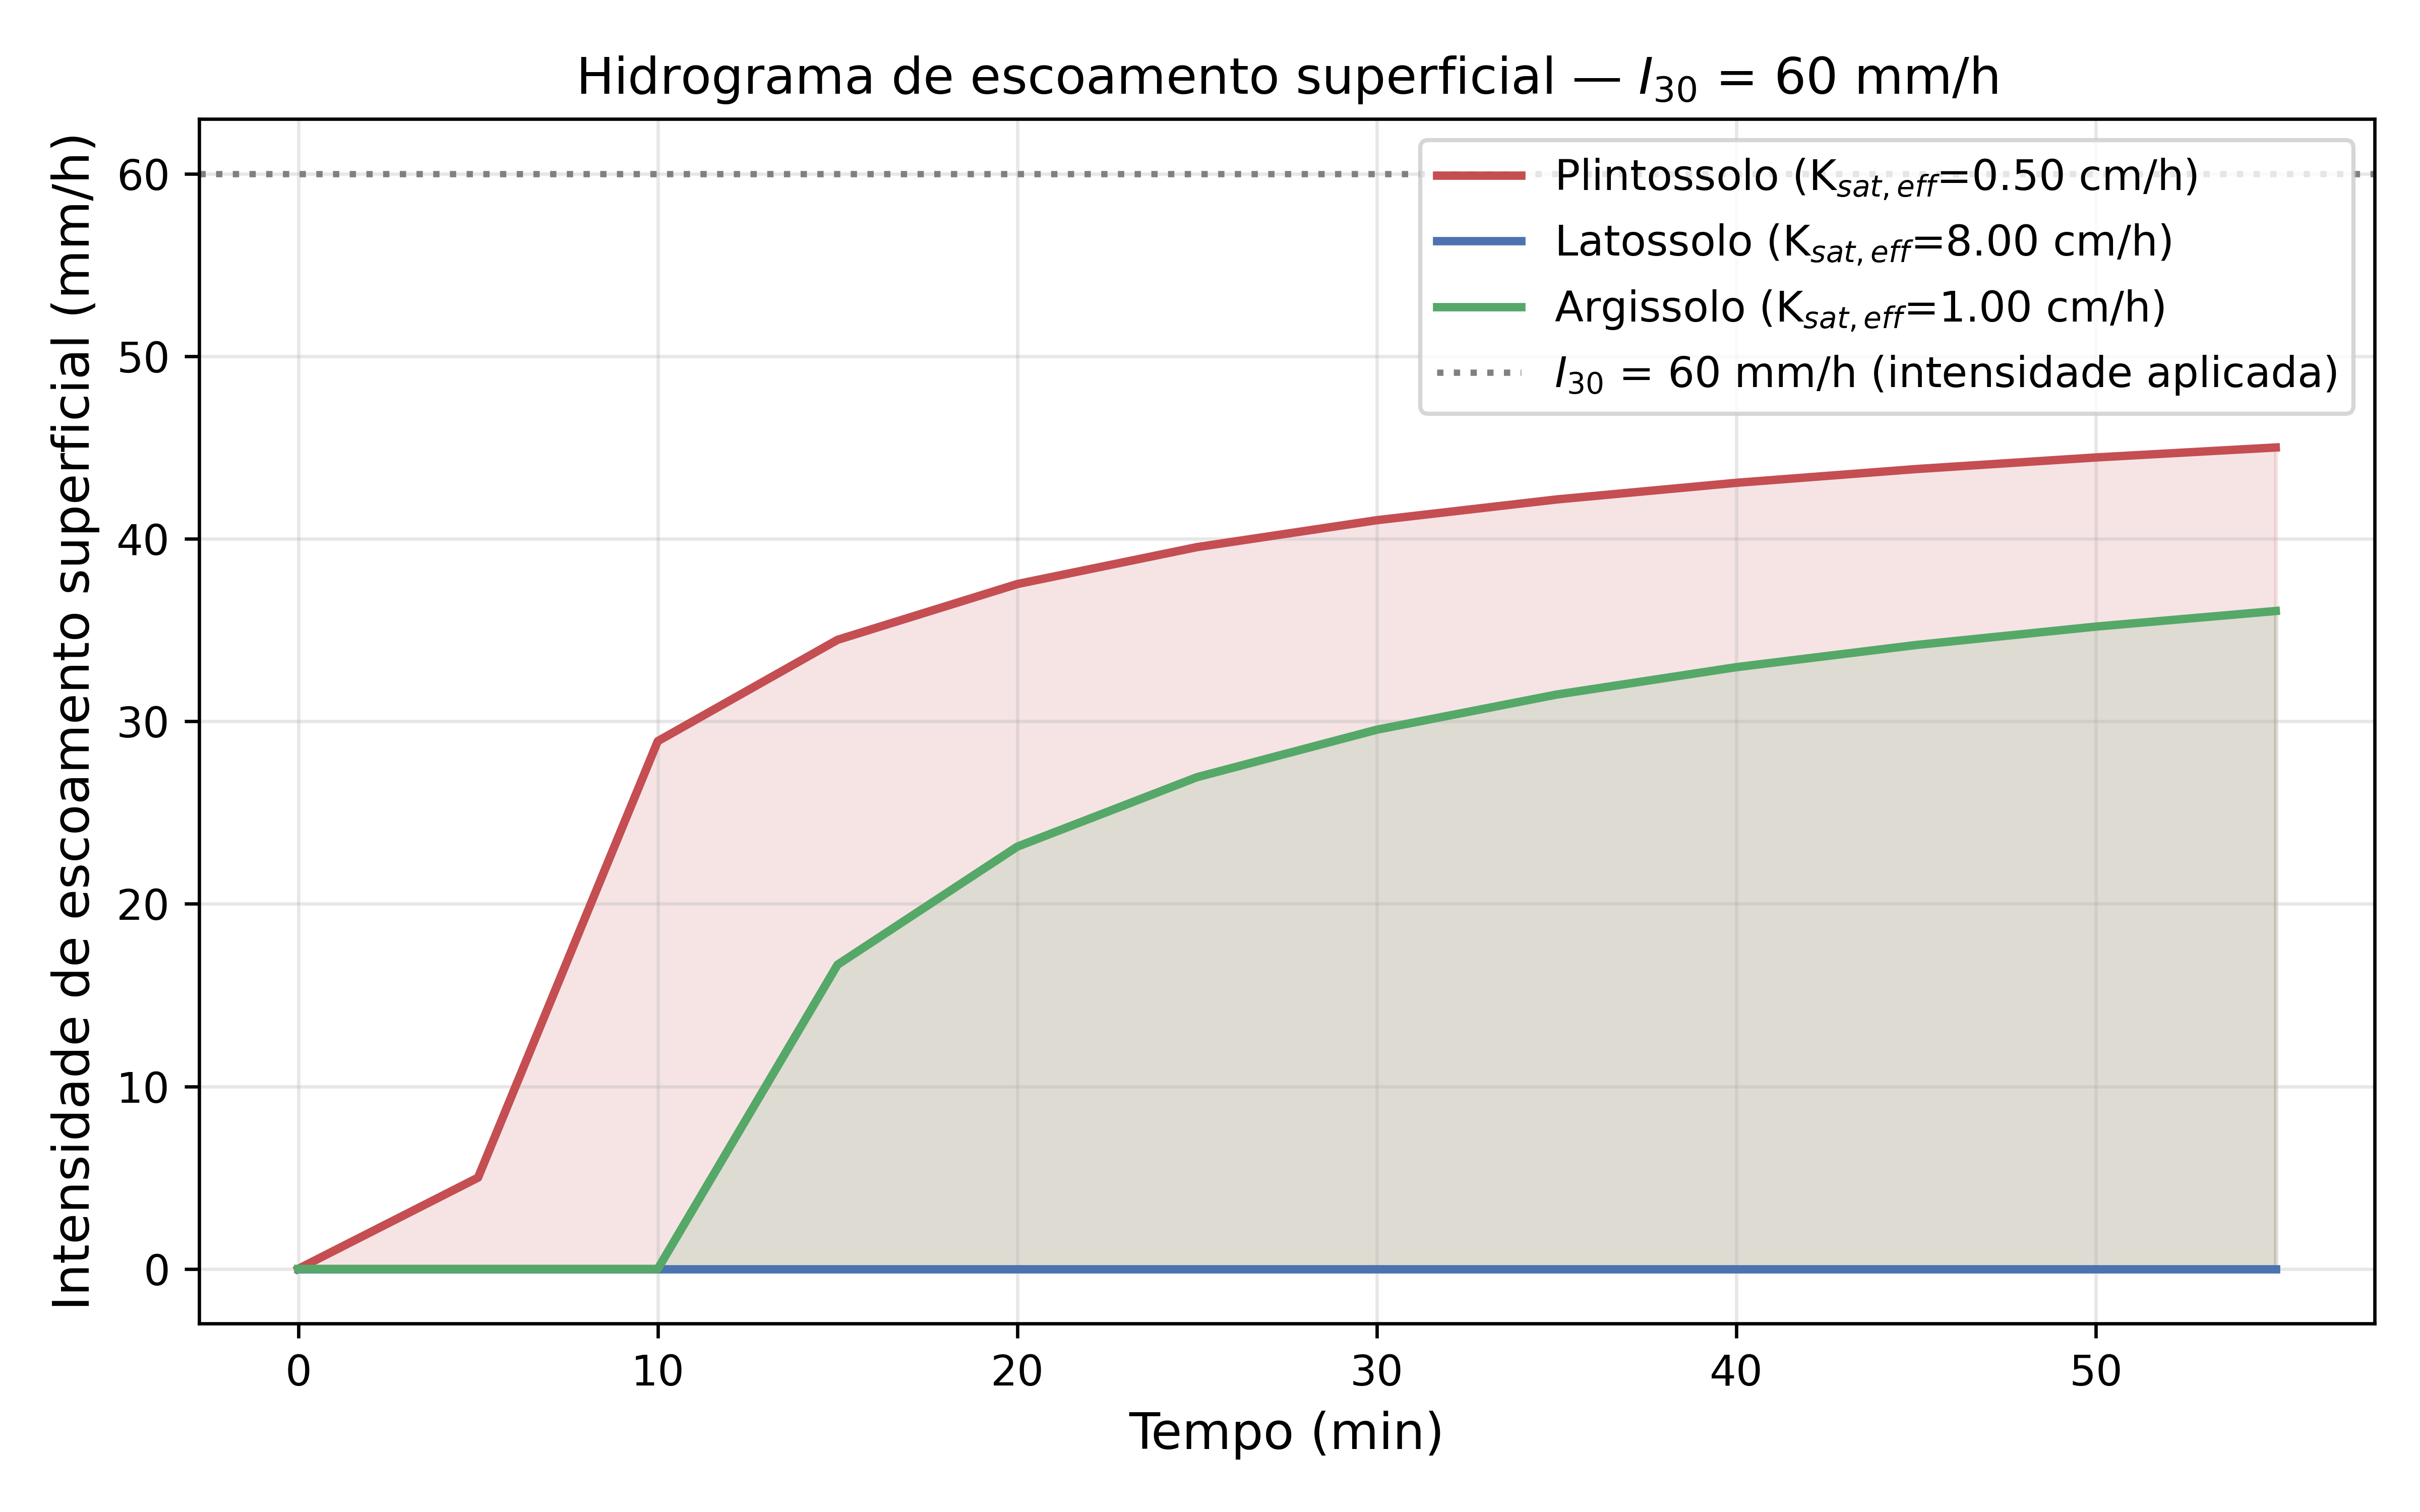
\includegraphics[width=0.8\textwidth]{figuras/fig_07_hidrograma_i60.png}
\caption{Surface-runoff hydrograph under maximum 30-minute intensity ($I_{30}$) of 60~mm/h for the three soil profiles. The Plinthosol (effective saturated hydraulic conductivity 0.50~cm/h) reaches steady state in less than 10~minutes, while the Ferralsol (8.0~cm/h) generates no runoff at any point during the 60-minute event.}
\label{fig:hidrograma}
\end{figure}

\subsection{Virtual erosion and \texorpdfstring{$\delta$}{delta} discrepancy (Test~5)}

The mean discrepancy $\delta_{\mathrm{obs}}$ for the Plinthosol ($2.71 \pm 0.91$ for $I_{30} \geq 40$~mm/h) fell below the $\delta_{\mathrm{mod}} = 8.01$ predicted with the uncalibrated target parameters, yielding a relative error of 66\% (Fig.~\ref{fig:erosao}c--d), an overestimation expected because the ``true'' parameters ($n_1 = 1.0$, $\beta_{\max} = 2.5$ etc.) were set within plausible ranges and do not represent the actual site. The same overestimation trend manifests in the Acrisol ($\delta_{\mathrm{obs}} = 0.61$ only for $I_{30} = 100$~mm/h, versus $\delta_{\mathrm{mod}} = 2.29$), while the absence of erosion in the Ferralsol ($\delta_{\mathrm{obs}}$ indeterminate due to zero numerator) is consistent with $\delta \approx 1$ predicted by the model, reinforcing the pedological specificity of the correction factor.

A second source of discrepancy lies in the simplified detachment model ($D = k_r(\tau - \tau_c)$), which does not incorporate transport-capacity limitation and may underestimate $K_{\mathrm{obs}}$ for extreme events in which sediment is transported out of the plot before accumulating. \citet{nearing_nicks_1998} observed analogous behaviour when evaluating WEPP on experimental slopes, where predicted erosion systematically exceeded measured erosion in high-intensity events when transport capacity was not imposed as a limiter. Complementarily, \citet{deviren_saygin_et_al_2018} demonstrated that process-based detachment erodibility tends to diverge from empirical USLE erodibility in soils with high dispersible-clay fractions, a category that includes Plinthosols owing to the presence of kaolinite and low structural stability in subsurface horizons.

\begin{figure}[htbp]
\centering
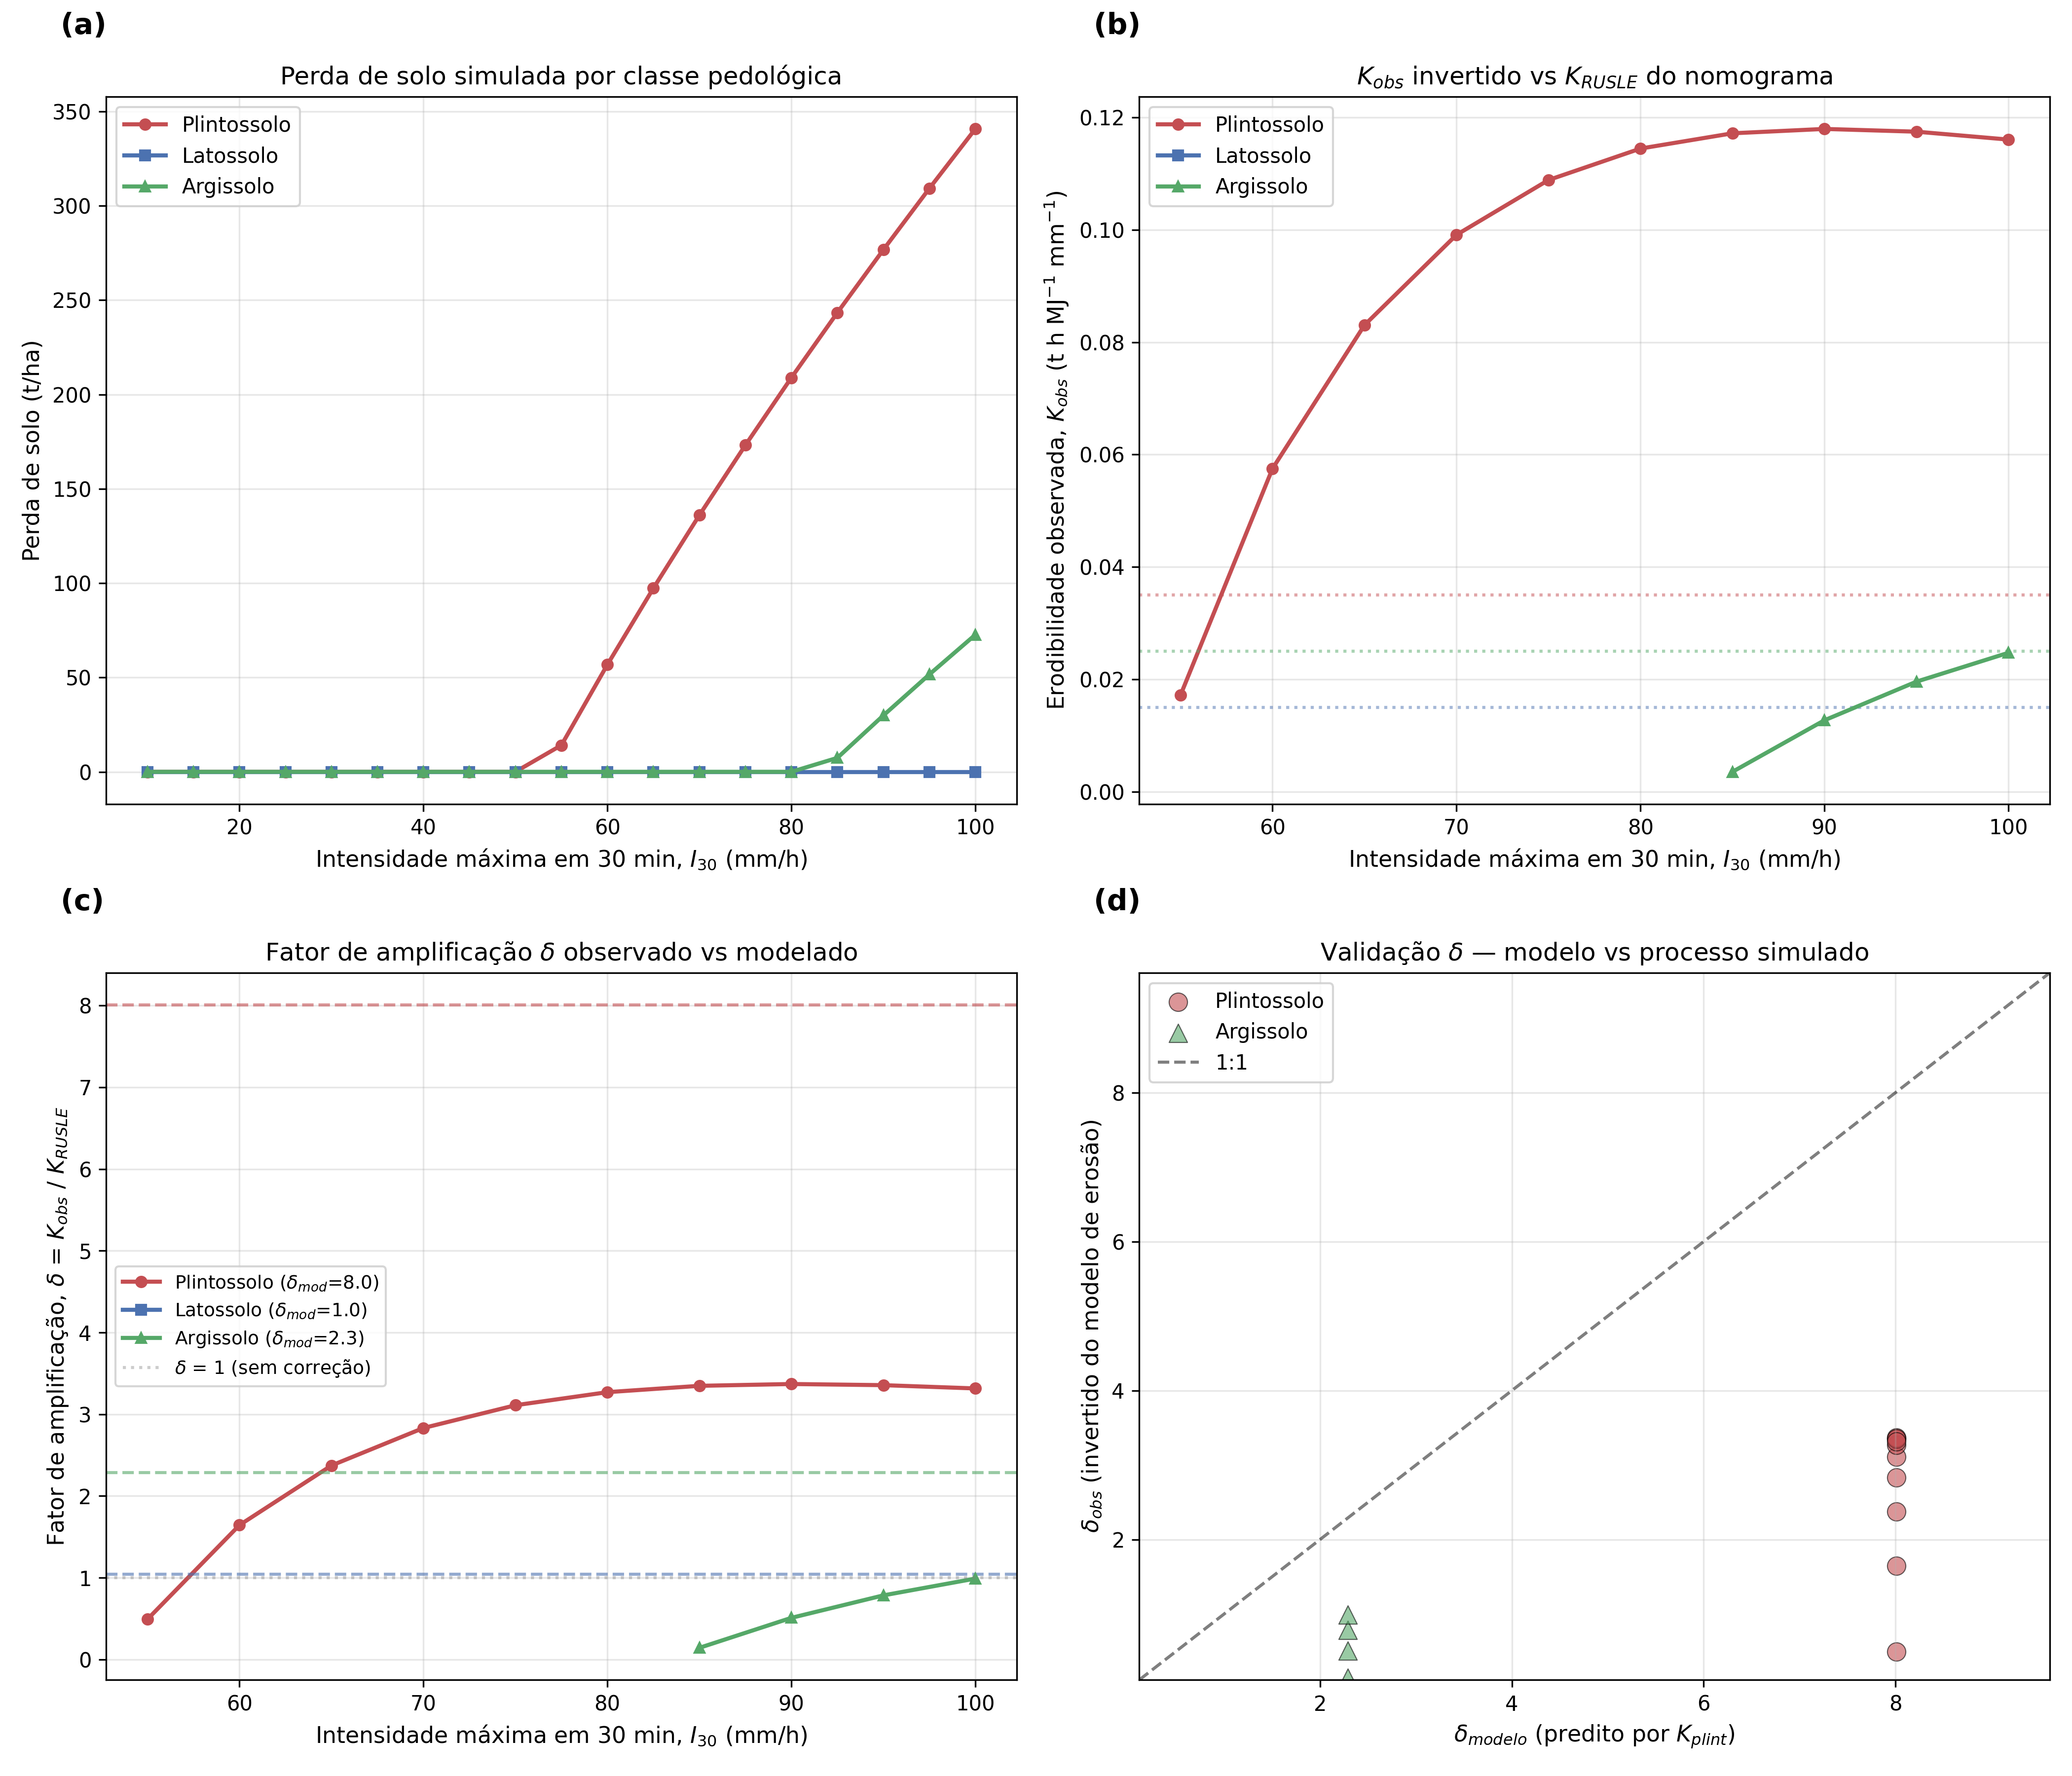
\includegraphics[width=\textwidth]{figuras/fig_08_erosao_virtual.png}
\caption{Results of the virtual erosion simulation (WEPP-type detachment model). (a)~Soil loss by pedological class and maximum 30-minute intensity ($I_{30}$). (b)~Observed erodibility ($K_{\mathrm{obs}}$), inverted via the USLE relation, compared with nomograph erodibility ($K_{\mathrm{RUSLE}}$, dotted lines). (c)~Observed amplification factor ($\delta_{\mathrm{obs}} = K_{\mathrm{obs}}/K_{\mathrm{RUSLE}}$) as a function of $I_{30}$, with modelled amplification ($\delta_{\mathrm{mod}}$) as reference (dashed lines). (d)~Validation $\delta_{\mathrm{obs}}$ versus $\delta_{\mathrm{mod}}$ (1:1 line).}
\label{fig:erosao}
\end{figure}

Despite the parametric overestimation, the $K_{\mathrm{plint}}$ model preserves the pedological hierarchy (Plinthosol $>$ Acrisol $>$ Ferralsol) and generates $\delta$ values structurally consistent with the simulated processes, a result coherent with the premise that the multiplicative structure captures the relative contribution of each amplifying mechanism even when the absolute parameter values are uncalibrated \citep{renard_et_al_1997}. The $K_{\mathrm{obs}}$ values of 0.058--0.116~t\,h\,MJ$^{-1}$\,mm$^{-1}$ obtained for the Plinthosol lie in the upper range of erodibility documented for Brazilian soils with limiting subsurface horizons \citep{lafayette_cantalice_coutinho_2011,cassol_et_al_2023} and exceed the original nomograph estimates by 2--8 times \citep{wischmeier_et_al_1971}, a pattern consistent with the systematic underestimation reported by \citet{alewell_et_al_2019} for tropical soils with dominant subsurface processes. \citet{torri_poesen_2014} had already indicated that erodibility is an emergent property of the profile rather than solely of the surface horizon, an argument that supports the need for correction factors integrating pedological information at depth.

The compatibility with values measured by \citet{bagarello_et_al_2012} on experimental plots in Sicily (0.040--0.090~t\,h\,MJ$^{-1}$\,mm$^{-1}$) for soils with a subsurface clay horizon is relevant despite the climatic contrast between the semi-arid Mediterranean regime (precipitation concentrated in short-duration events) and the humid tropical regime of the present site, because the common mechanism of textural discontinuity generates comparable hydraulic impedance in both contexts. \citet{ostovari_et_al_2016} observed analogous nomograph underestimation in calcareous soils with subsurface impedance in Iran, whereas \citet{francois_et_al_2024} identified the $K$ factor as the most sensitive RUSLE parameter in southern Bahia under pedoclimatic conditions similar to those of the present study. The convergence in orders of magnitude across contrasting geomorphological provinces suggests that the nomograph underestimates erosive susceptibility when subsurface processes govern the hydrological response of the profile, and that multiplicative correction factors such as the one proposed may have applicability beyond Plinthosols.

Field calibration with data from plots under natural rainfall can adjust the five parameters to minimise the distance between $\delta_{\mathrm{obs}}$ and $\delta_{\mathrm{mod}}$. Adoption of a Bayesian approach with geotechnical priors derived from the Rankine analysis may mitigate the residual equifinality of $k_3$ and $n_3$ identified in the parameter-recovery and global-sensitivity analyses, where these two parameters exhibited high dispersion and mutual interaction in the interval $H/H_c < 0.45$ \citep{beven_freer_2001}.

%% ================================================================
%%  5. CONCLUSIONS
%% ================================================================
\section{Conclusions}
\label{sec:conclusions}

The multiplicative formulation $K_{\mathrm{plint}}$ reproduced the susceptibility hierarchy among Plinthosol, Acrisol and Ferralsol in all tests, indicating that the three-term independent structure captures the relative contribution of each amplifying mechanism even prior to field calibration. The subsurface hydraulic impedance concentrated the largest share of amplification variance in the two classes with VIB below the reference threshold, a result coherent with the expectation that the Hortonian runoff regime governs the erosive response in stratified soils and with the systematic nomograph underestimation reported on tropical and Mediterranean plots. The Ferralsol, by combining favourable drainage, toxicity and geotechnical stability conditions, responded with amplification near unity in all realisations, validating the multi-class design as a prerequisite for isolating individual amplifying effects. The adopted basic infiltration rate threshold differentiated infiltration-dominated from runoff-dominated soils coherently with the Green--Ampt model, suggesting that this threshold may serve as an operational screening criterion for application of the correction factor.

The synthetic calibration confirmed that the three parameters governing hydraulic penalisation and edaphic toxicity are recoverable with reduced bias even under high noise, whereas the geotechnical parameters exhibited equifinality whose origin lies in the flattened response surface of $\gamma$ across the normalised depth range of the mapped features. Validation by the Rankine model indicated that this indeterminacy may be mitigated by incorporating physical constraints derived from slope stability as priors in the calibration, and that the geotechnical contribution remains secondary in the shallow gullies studied, becoming potentially relevant only in gullies with normalised depth exceeding the identified threshold. The separation between mechanistic interactions, such as the covariance between infiltration and toxicity, and purely parametric interactions, such as the compensation between scale and curvature of the geotechnical factor, guides the differential allocation of instrumental effort during the field phase.

The convergence between simulated erodibility values and the orders of magnitude documented on experimental plots in contrasting pedoclimatic contexts suggests that the nomograph underestimates erosive susceptibility recurrently when subsurface processes govern the profile response. The earlier onset of steady-state runoff observed in the Plinthosol hydrograph may have implications for the temporal dimensioning of erosion-control structures, an aspect warranting field investigation. Since the simulations were conducted with profiles parameterised from the literature, definitive validation depends on calibration with data from plots under natural precipitation, and extension of the model to other classes with restrictive subsurface diagnostics remains conditional on empirical verification of the independence among the three amplifying terms.

%% ================================================================
%%  BACKMATTER
%% ================================================================
\backmatter

\bmhead{Acknowledgements}

The author thanks the Departamento de Zootecnia of Universidade Federal de Sergipe for logistical support and CAPES for the postdoctoral fellowship.

\section*{Declarations}

\bmhead{Conflict of interest} The authors declare that they have no known competing financial interests or personal relationships that could have appeared to influence the work reported in this paper.

\bmhead{Data availability} The simulation scripts, input parameters and generated figures are available at Zenodo (\url{https://doi.org/10.5281/zenodo.19483403}).

\bmhead{Funding} CAPES postdoctoral fellowship.

\bmhead{Author contribution} E.G.S. conceived and implemented the model, conducted the simulations, analysed the data and wrote the manuscript.

\bibliography{../referencias_artigos}

\end{document}
